\documentclass{acm_proc_article-sp}
\usepackage[utf8]{inputenc}

\renewcommand{\paragraph}[1]{\vskip 6pt\noindent\textbf{#1 }}
\usepackage{hyperref}
\usepackage{graphicx}
\usepackage{url}

\providecommand{\tightlist}{%
  \setlength{\itemsep}{0pt}\setlength{\parskip}{0pt}}

\title{Knowledge Ecosystem - Deep Learning and Education}


% Add imagehandling
\usepackage{graphicx}
% Redefine \includegraphics so that, unless explicit options are
% given, the image width will not exceed the width of the page.
% Images get their normal width if they fit onto the page, but
% are scaled down if they would overflow the margins.
\makeatletter
\def\ScaleIfNeeded{%
  \ifdim\Gin@nat@width>\linewidth
    \linewidth
  \else
    \Gin@nat@width
  \fi
}
\makeatother
\let\Oldincludegraphics\includegraphics
{%
 \catcode`\@=11\relax%
 \gdef\includegraphics{\@ifnextchar[{\Oldincludegraphics}{\Oldincludegraphics[width=\ScaleIfNeeded]}}%
}%

\numberofauthors{2}
\author{
\alignauthor Fanli (Christian) Zheng \\
        \affaddr{dyad x machina}\\
       \email{\href{mailto:thechristianramsey@gmail.com}{\nolinkurl{thechristianramsey@gmail.com}}}
\and \alignauthor Haohan Wang \\
        \affaddr{dyad x machina}\\
       \email{\href{mailto:haohan723@gmail.com}{\nolinkurl{haohan723@gmail.com}}}
\and }

\date{{[}DRAFT{]} 2018-11-20}

%Remove copyright shit
\permission{}
\conferenceinfo{} {}
\CopyrightYear{}
\crdata{}

% Pandoc syntax highlighting


\begin{document}
\maketitle


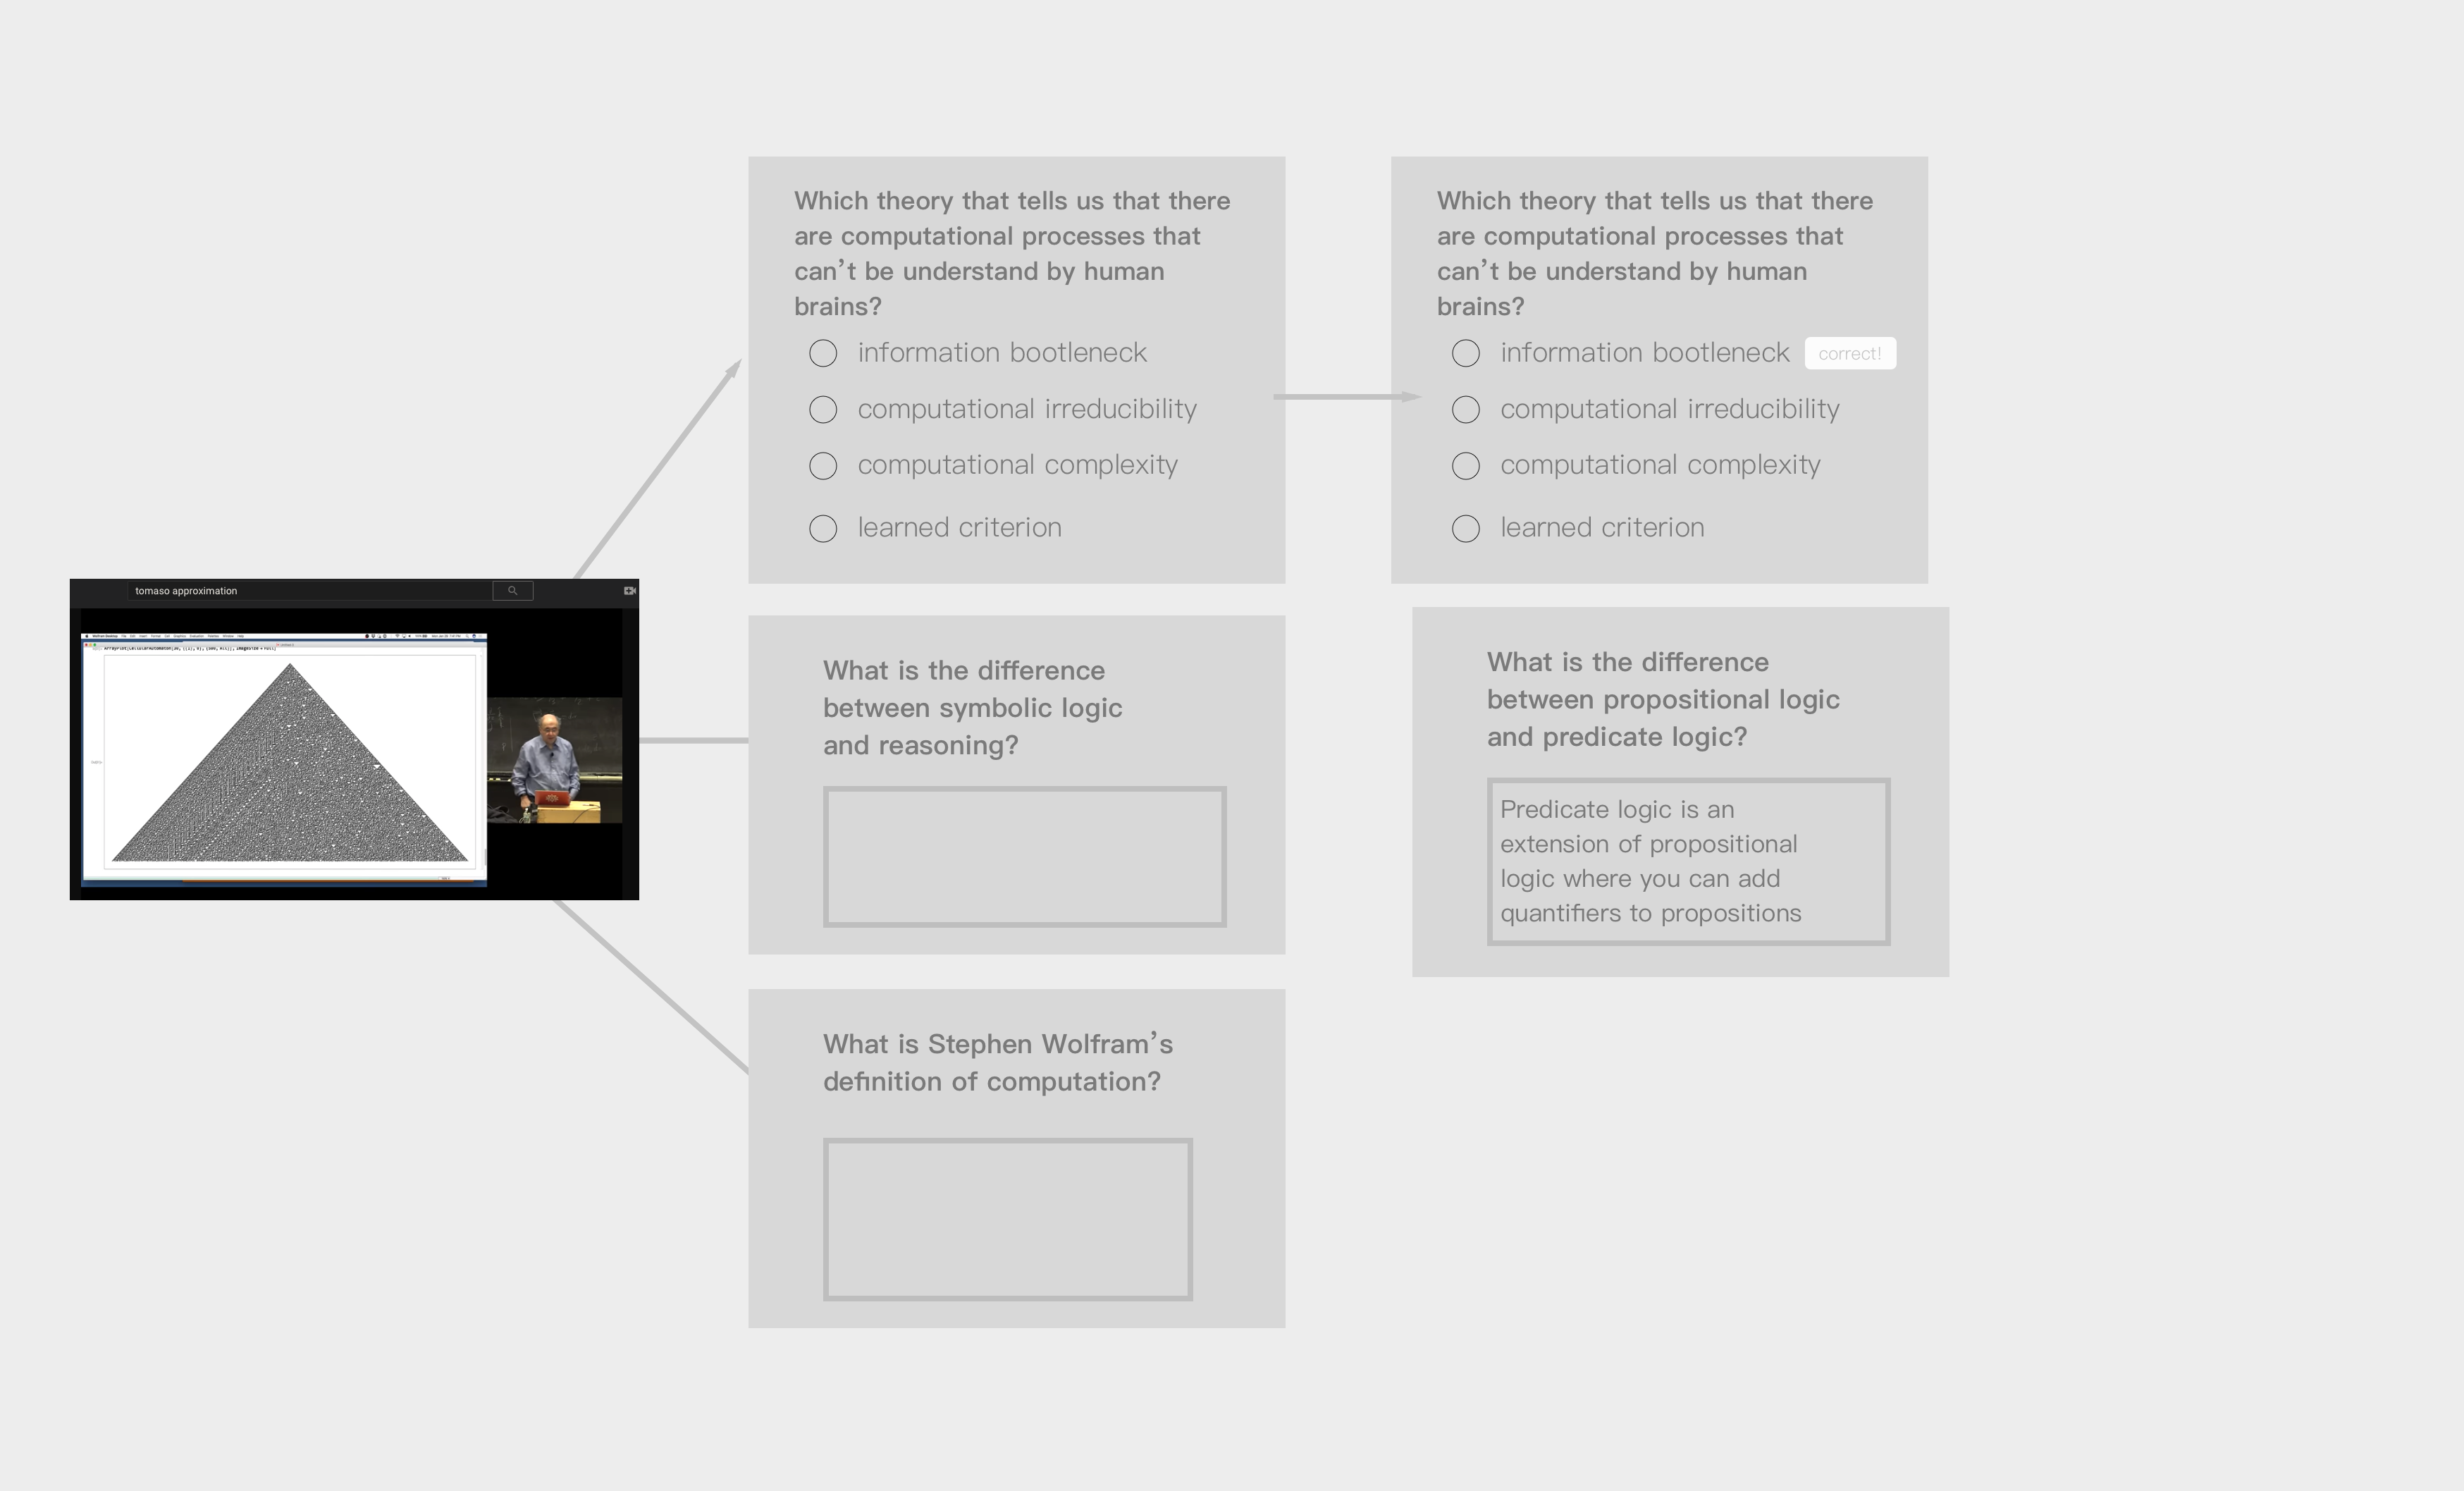
\includegraphics{img/MtoQA.png}
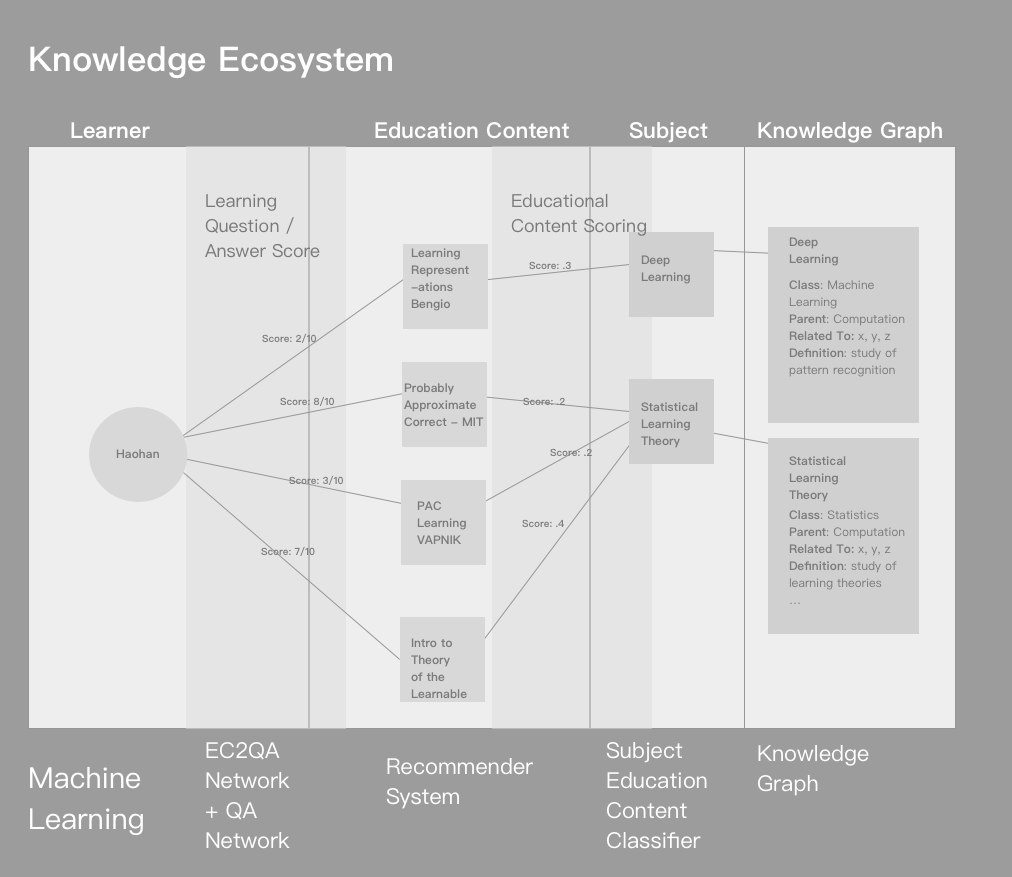
\includegraphics{img/knowledgeEcosystem.png}

\hypertarget{mc_embed_signup}{}
\hypertarget{mc_embed_signup_scroll}{}
We are looking for educators, researchers, and designers to collaborate.
Send us your email to stay updated

Email Address *

\hypertarget{mce-responses}{}
\hypertarget{mce-error-response}{}

\hypertarget{mce-success-response}{}

\chapter{Introduction}\label{introduction}

\begin{figure}
\centering
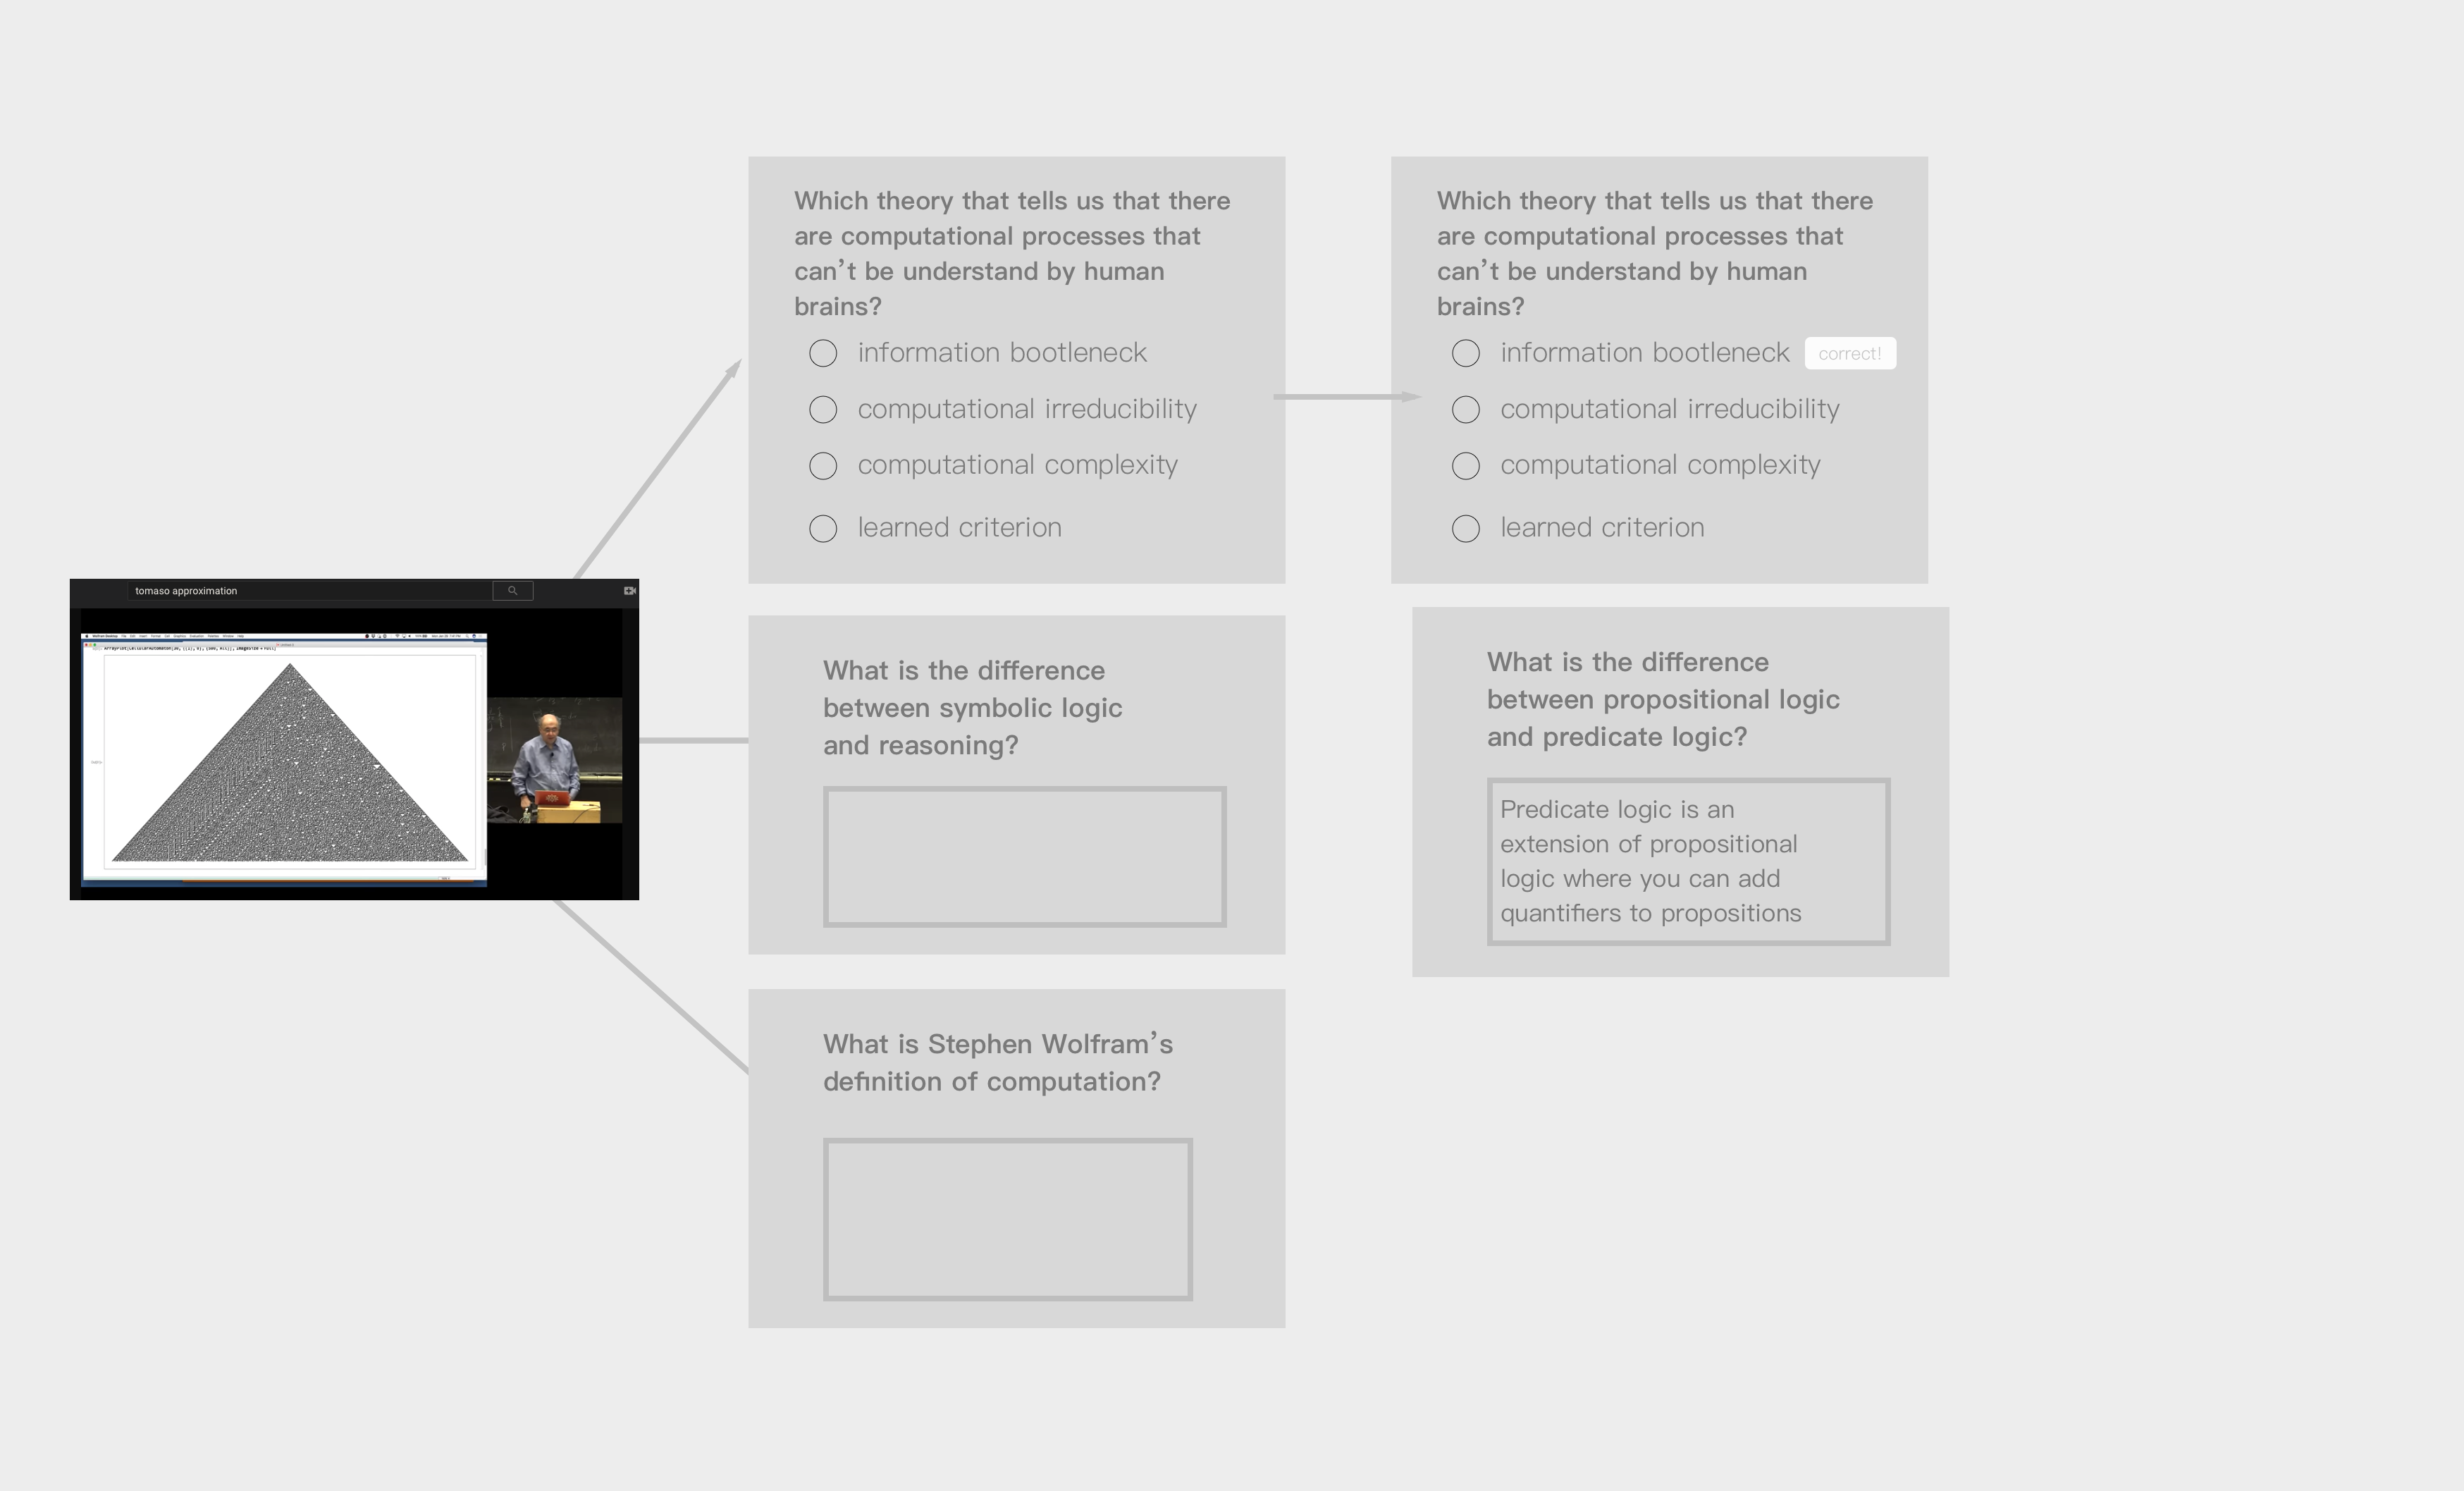
\includegraphics{img/MtoQA.png}
\caption{EC2QA Network}
\end{figure}

\section{A Future}\label{a-future}

Let's start with a future view of an individual's education. Many of us
have used the internet to educate ourselves with the abundance of medium
to high quality videos, papers, articles, podcasts and how-tos being
uploaded from numerous individuals, groups, and institutions like never
before (60 hours of video are uploaded to youtube.com every minute).

Let us imagine that all of what you have learned online, throughout the
entirety of your life, from the hundreds of Youtube videos, Wikipedia
articles, Nature papers, and podcasts you've read, watched, or listened
to, were all added structurally to your \textbf{knowledge journey}, and
what if that journey could be consolidated into what we might call a
\textbf{knowledge footprint} that could be shared with others? Could
this replace static degrees? Or augment them to be more inclusive of a
learner's true knowledge? How might we test such knowledge? Could we
even predict and provide the guidance on what an individual should be
learning next to best support their knowledge acquisition?

\section{A Comparison}\label{a-comparison}

Now, let's go back to our current approach to education. Many of us
treat knowledge acquisition like a chapter in the individual's life that
is limited to one or more formal places i.e.~universities. This is
misleading since we accrue knowledge from everywhere and most recently
the internet has become a primary source of knowledge acquisition but
has gone mostly unaccounted for in terms of recognition (i.e.~watching a
whole series of Youtube lectures on the Neurobiology of Depression or
Discrete Mathematics goes mostly unnoticed when someone views one's
resume or by simply looking at their degree). The current approach makes
it much harder for people to switch to working and exploring the domains
or professional fields outside of their degree area. Knowing rigourous
mathematics and not having a degree in it, is said to be surprising,
therefore the current ``thumbnail view'' of an individual's knowledge is
necessarily inadequate to the new mediums of knowledge acquisition.

\begin{figure}
\centering
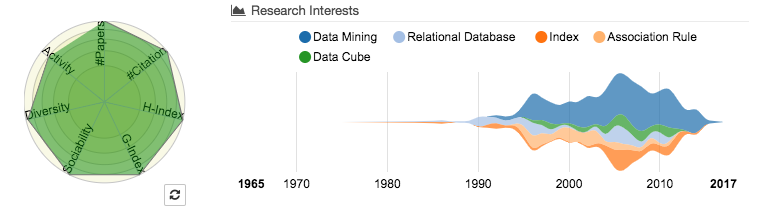
\includegraphics{img/aminer.png}
\caption{Example at aminer.com}
\end{figure}

The ideas behind this \emph{knowledge ecosystem}, presents only one of
many possible solutions to bringing our education system into modernity.
The goal of it would be to promote the long held idea of the
\textbf{life-long learner}. Moving away from the ``education chapter''"
of an individual's life to the individual as an evolving learner;
learning the necessary skills for what life presents them with today or
might tomorrow. It would (combined with traditional education) show us a
more accurate depiction of a learner's knowledge and therefore that of a
society's collective knowledge.

Visualised over time, we could begin to capture a learner's so called
\textbf{knowledge journey}. Composed of every piece of content they've
gained knowledge from mapped to the \emph{human knowledge graph}.
Showing how an individual has traversed through the world of human
knowledge.

This would also serve as a way for others, who may be on a similar
\textbf{knowledge journey} to connect with ``their'' cohort which may
not need to be bounded by geography or demography. This could be the
start of meetups, study groups, flexible class models and so on.

For those who are looking for a change, they may find different journeys
that help them decide what step to take next. You would also be able to
connect someone's occupation to their \textbf{knowledge journey}.

On aggregate, we could begin to cluster similar \textbf{knowledge
journeys} through unsupervised learning, which might lead to completely
new journeys that others may be inspired to follow.

\section{Knowledge Ecosystem}\label{knowledge-ecosystem}

In this essay, we will propose a \textbf{knowledge ecosystem}, a new way
of approaching education that attempts to build a more accurate
depiction of a learner's true knowledge. It will require significant
effort to bring to life but we believe the benefits will outweigh the
costs. We will talk about how we can use machine learning, deep learning
in particular, to help create and support a \textbf{knowledge ecosystem}
which is made up of the learner's \textbf{knowledge footprint},
\textbf{knowledge journeys}, and a \textbf{collective human knowledge
graph}. We will introduce current advances in deep learning that would
enable us to take the space of unstructured educational content on the
web and do the following,

\begin{itemize}
\item
  classify content to higher level subjects
\item
  map content unto the human knowledge graph
\item
  test a learner's knowledge of recently viewed educational content
  through questions and answers, no what matter the subject.
\end{itemize}

We will also argue that this imagined future is not only
\textbf{desirable} for society but something similar is required to
ensure individual's knowledge are well represented in a time where the
pace of change is rapidly speeding up.

Let us not forget, that even software engineering is currently being
recreated with machine learning as a key pillar which wasn't much of a
thought 5-10 years ago.

It is going to be tantamount if we have an adaptive systems that can
represent our current knowledge and also make us predictable to others
given the future pushes us to knowing more than ever and knowing who to
collaborate with to apply such knowledge.

This hypothetical future isn't just conceptual, most of what we will
present to you today is currently feasible due to the most recent
advances in machine learning, and in particular deep learning

In the last section of this essay I will review what has been proposed
and also call other researchers, teachers, and designers to collaborate
on such an ecosystem, even if it is just in part.

*Note: For the purpose of this essay we will talk mostly about digital
knowledge acquisition and leave the reader to extend the basics to
knowledge obtained elsewhere.

\chapter{Primary Concerns}\label{primary-concerns}

There are 3 main concerns that we will attempt to address in this
article about online knowledge acquisition that stand in the way of
having an adaptive and reliable knowledge ecosystem. We will attempt to
present a system that can sufficiently overcome each of the concerns
here and in the implementation section.

There are as follows:

\begin{itemize}
\item
  \textbf{Passive Consumption} - most of online content is viewed
  passively by the learner and the result of passive consumption is that
  learner's do not grasp the concepts or master the content being
  taught.
\item
  \textbf{Untested Knowledge} - even if the learner was engaged while
  viewing a piece of educational content their knowledge is untested and
  therefore it isn't clear if they've mastered the content accurately
  and in some sense holistically.
\item
  \textbf{Knowledge Representation} - even if the learner was engaged
  (1) and their knowledge was tested (2), simply knowing the counts or
  types of video they watched doesn't make their knowledge predictable
  and useful to others. In fact, even the learner may be unaware of all
  of what they've viewed.
\end{itemize}

\section{Passive Consumption and Untested
Knowledge}\label{passive-consumption-and-untested-knowledge}

\begin{quote}
How would such an ecosystem insure us against passive consumption?
\end{quote}

\textbf{Scenario \#1} A learner goes online and begins watching a series
on Machine Learning. How do we engage and test a user's knowledge?

\emph{Proposition:} Using advances in deep learning, we propose a dual
question and answer generation framework given the educational content.

\emph{Result:} A learner gets a set of questions and multiple choice
answers throughout the video. Keeping the user engaged and sharp to
ensure they can answer each of the questions.

As you can see, we've bundled passive consumption and untested knowledge
because our proposed ecosystem approaches both of these by always
testing knowledge. We will show the current research results in deep
learning in the implementation section.

\section{Knowledge Ecosystem Example}\label{knowledge-ecosystem-example}

\begin{figure}
\centering
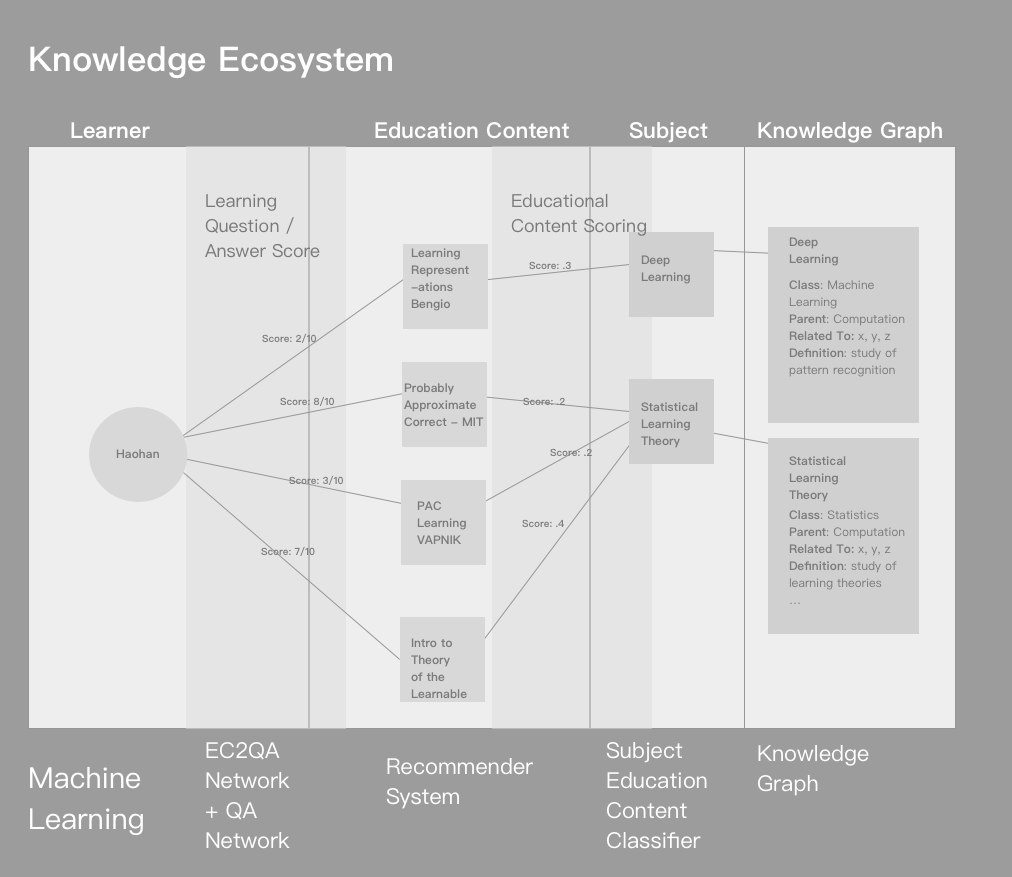
\includegraphics{img/knowledgeEcosystem.png}
\caption{Knowledge Ecosystem}
\end{figure}

Given a piece of educational content, our knowledge system will generate
a set of questions and answers that theoretically capture the major
concepts and facts that the learner should know after viewing a part or
the content in whole.

You can imagine watching a Youtube video and after a learner views 15
minutes of an hour long lecture on computational complexity a quiz is
presented (i.e.~a set of questions and answers conditioned on the past
15 minutes of video), and the results are recorded. In the future we
would also be able to use the knowledge graph to bring in learner's
existing knowledge in order to generate more complex questions and
answers based on his/her previous knowledge and the current educational
concepts.

As the first step, our knowledge system would only consider content that
has been watched with some engagement for now.

\section{The Problem of Knowledge
Representation}\label{the-problem-of-knowledge-representation}

\begin{quote}
Given most learner's online knowledge acquisition varies and has been
invisible up to now, how we can best represent their knowledge?
\end{quote}

\textbf{Scenario \#2} A learner has a degree in Public Health, but since
graduating, he has been studying machine learning for the last 3 years.
The learner now wants to apply to a job that requires Health and Machine
Learning. How do we represent their traditional and updated knowledge?

This is a tricky problem that goes beyond any given algorithm. The exact
design of a \textbf{knowledge footprint} and a \textbf{knowledge
journey} has been attempted and we will not cover that in depth here.
The proposed system presupposes the design of the knowledge footprint.

There is another problem:

\begin{quote}
how do we reduce someone's knowledge (in this case a set of educational
content and their respective scores) into a symbol that is
representative of his/her current knowledge and could be shared across?
\end{quote}

\emph{Proposition:} We introduce \textbf{knowledge journeys} and the
\textbf{knowledge graph} as a way to make sense and structure a
learner's knowledge acquisition. The collective \textbf{knowledge graph}
will tell us about the subject the learner is studying and we can use
this to compare to others and create a relative comparison.

\emph{Result:} Reducing a learner's \textbf{knowledge journey} into a
common set of dimensions that makeup into their \textbf{knowledge
footprint} which would look similar to those with similar journeys.

As a result, the employer, now familiar with the footprints can check
the overlap between the current employee's and a prospective employee's
to support their decision making.

\chapter{Concepts}\label{concepts}

As mentioned above, we will be introducing a few novel concepts that we
believe are the key components of such an educational ecosystem.

\section{Knowledge Footprint}\label{knowledge-footprint}

The concept of a knowledge footprint is a custom symbol or badge with a
profile that represents one's education relative to that of others. This
concept is particularly designed for solving the second the knowledge
representation concern that we proposed earlier.

In turn, this footprint should be able to represent all of one's
education (currently focused on digital) while balancing distinction and
commonality with others.

\emph{This example from Aminer is a good visual for a knowledge
footprint and journey.} 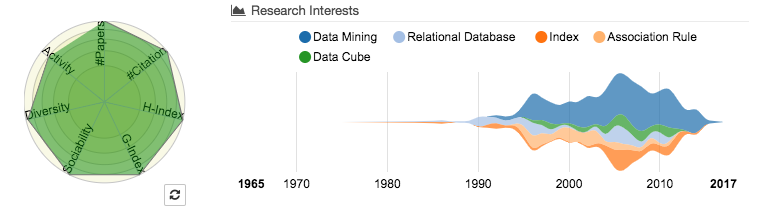
\includegraphics{img/aminer.png}

\section{Knowledge Journeys}\label{knowledge-journeys}

\begin{figure}
\centering
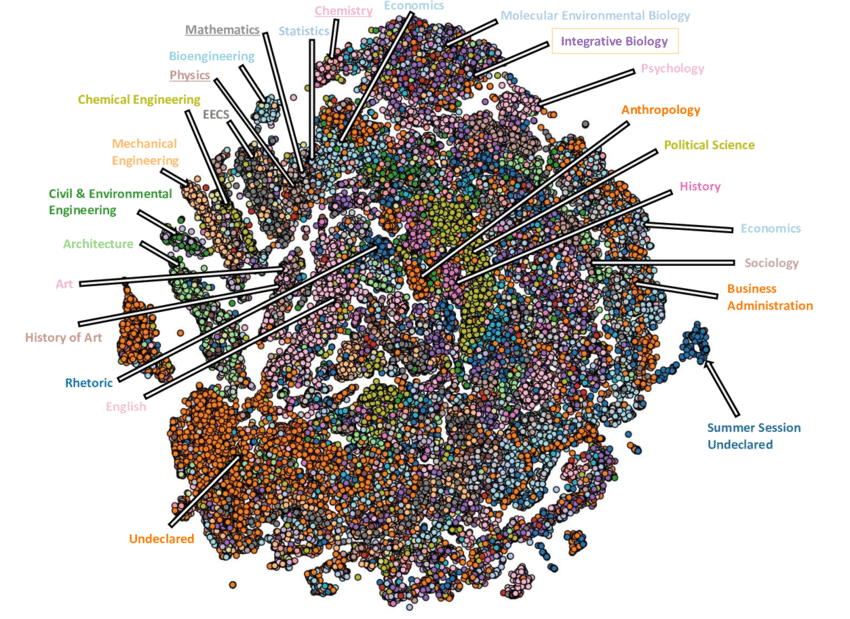
\includegraphics{img/tsne.png}
\caption{Image title}
\end{figure}

Image src:
\url{https://www.researchgate.net/figure/t-SNE-projection-of-the-embedding-of-all-learners-in-the-dataset-Major-labels-are_fig1_323391033}

A \textbf{knowledge journey} is a somewhat holistic view of all of the
educational content a learner has acquired over time. The journey should
be a temporal representation of all of the subjects that one has viewed
and been tested on. Knowledge journey should be simple enough to
comprehend and compare but complex enough that the individual can go
back to any particular moment in time and review the educational content
they've viewed before. Coupled with the knowledge graph, it can also
shed light on the possible next education content that a learner should
be or would be interested learning.

This concept also helps address the knowledge representation concern.
This time instead of capturing a consolidated snapshot of one's current
knowledge, this concept takes a temporal route to capture one's entire
learning path.

\section{Collective Human Knowledge
Graph}\label{collective-human-knowledge-graph}

\begin{figure}
\centering
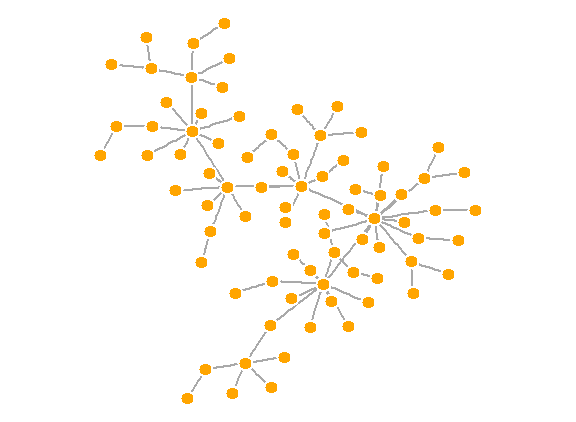
\includegraphics{img/knowledge_graphy.png}
\caption{Image title}
\end{figure}

The collective human knowledge graph can be compared to Google's Search
Knowledge Graph {[}{\textbf{???}}{]} which points unstructured
information towards structure. The graph should have all existing
subjects that we are currently aware of (i.e.~Mathematics, Computer
Science, Art, and Sociology, etc). Since each piece of educational
content will be classified into one more more sub-subject(s), all
subjects will exist in detail within the knowledge graph.

On the other hand, we could also use these subjects that are associated
with that piece of content to help create the knowledge footprint for
the learner.

\section{EC2QA Network}\label{ec2qa-network}

We mentioned the EC2QA network earlier because currently we would have
to cobble together multiple networks to make this work. Instead we will
introduce a novel network framework, EC2QA, to solve the problem of
generating questions and answer pairs for any given educational content
(text, video, image, pdf, etc).

The possible implementation solutions are introduced in the
implementation section.

\section{Knowledge Ecosystem by
Example}\label{knowledge-ecosystem-by-example}

\begin{figure}
\centering
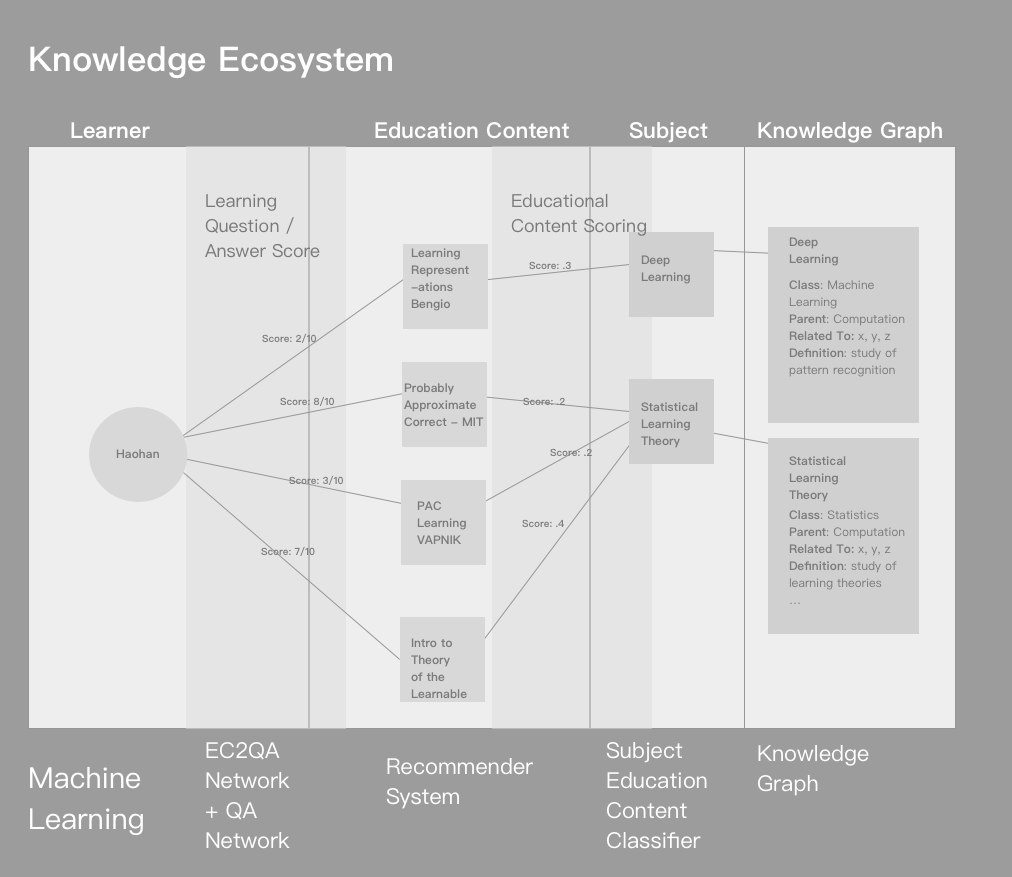
\includegraphics{img/knowledgeEcosystem.png}
\caption{Knowledge Ecosystem}
\end{figure}

Now that we are aware of each of the elements, let's talk about how they
work in practice.

A learner watches a video titled `Depression' by Robert Sapolsky.

\begin{itemize}
\item
  The video is classified by a neural network as the following subjects
  {[}Neuroscience, Mental Health, Psychology{]};
\item
  The subjects are then mapped to the \textbf{knowledge graph} which
  gives us more information about each subject;
\item
  Using EC2QA or similar, a set of questions and answers are generated
  for every 15* minutes of video;
\end{itemize}

A learner is present with 5 questions to answer and scores 4/5 (80\%).

\begin{itemize}
\tightlist
\item
  The link between user and video takes up the score;
\end{itemize}

At the end of the video, the learner records a video summary and is
evaluated with a score 7/10 (70\%).

\begin{itemize}
\item
  The evaluation network looks at the \textbf{semantic and conceptual
  mutual information} shared between the original content and the
  learner's video summary;
\item
  All scores are mapped to the video and also counted at the subject
  level;
\end{itemize}

A learner looks at their knowledge footprint.

\begin{itemize}
\tightlist
\item
  All scores should be calculated against all subjects coming from the
  knowledge graph and compared against other learners to generate the
  footprint.
\end{itemize}

\chapter{Implementing the Knowledge
Ecosystem}\label{implementing-the-knowledge-ecosystem}

In this section, we set out to answer the following question:

\begin{quote}
How might we approach designing such a knowledge ecosystem?
\end{quote}

We will take a tour through a relevant set of implementations of the
elements within the proposed knowledge ecosystem. We will present the
relevant research in machine learning for each of the elements and also
propose a new artificial neural network architecture, Educational
Content to Question Answer (EC2QA) network, with the details needed to
design such a network.

\section{Problem Formulation}\label{problem-formulation}

Building such a knowledge ecosystem is not a trivial task. A necessary
step of searching for the proper solutions would be trying to break the
whole system into independent elements that we can deal with separately.
As we discussed earlier, we've divided the ecosystem into the elements
below:

\begin{enumerate}
\def\labelenumi{\arabic{enumi}.}
\item
  \textbf{Learning + Feedback} -- given a learner views a single
  educational content, reliably evaluate their knowledge and provide
  feedback for improvement to support learning (credibility, rigour)
\item
  \textbf{Knowledge Graph} -- relate any educational content to a
  concept which belongs to a particular subject, (relatibility,
  predictability)
\item
  \textbf{Knowledge Journeys} -- given educational content, a learner's
  score on such content, and history of viewing and testing, use the
  knowledge graph to map the learner's journey over time, offer a way
  for a learner to compare, connect with, and follow another's journey
  (compare, traverse)
\item
  \textbf{Knowledge Footprint} -- given a learner's journey, collapse it
  into a representative symbol(s) (relatibility, stable but evolving
  system )
\end{enumerate}

Much of element two (\#2) and element one (\#1) are possible with the
recent breakthroughs in the machine learning subfield, deep learning.
Elements three (\#3) and (\#4) may require a different approach to tie
the other elements together and there isn't a solution that ties each of
the elements together to our knowledge. We see \#3 and \#4 as design
problems to be approached from the bottom up. In this section we will
focus on the first two (\#1 \& \#2) elements.

\subsection{Before we start\ldots{}}\label{before-we-start}

As discussed above, recent trends in deep learning have produced
state-of-art results on relevant tasks that we will cover below.

To best illustrate the problem and possible solutions, to simplify our
examples we will focus solely on educational videos (Youtube or how-to
videos). Keep in mind that our ultimate goal is to apply our approach to
any type of online educational content including open texts, digital
texts, audio or podcasts.

Let us now explore some of the recent results that would enable us to
design the first two (\#1 \& \#2) elements of our ecosystem.

\section{Learning + Feedback}\label{learning-feedback}

\subsection{Question Formulation}\label{question-formulation}

In short, in this section we will be providing some insights on how to
solve the following puzzle:

\begin{quote}
``how can we take a single educational content and properly test a
learner's knowledge while also providing insightful feedback to support
their learning?''.
\end{quote}

\subsection{The Approach}\label{the-approach}

We consider learning + feedback as a key component of the ecosystem
which would settle our concerns with the issues of passive knowledge
consumption and untested knowledge.

Based on the above concerns we'll take a novel approach to ensure that
our learning + feedback element can do the following:

\begin{enumerate}
\def\labelenumi{\arabic{enumi}.}
\item
  Generate a set of questions and answers for any educational content
  (Domain: Question and Answer Generation)
\item
  Evaluate closed and open ended answers (Domain: Answer Evaluation)
\item
  Provide a score for the content based on the learner's performance
  (Domain: Aggregate scoring)
\end{enumerate}

The ideal result is to provide a learner with a credible picture of
their tested knowledge and an interactive learning experience that best
support their knowledge acquisition.

We will now explore some current research trends in deep learning that
will help us solve the problem.

In previous years, deep learning research has taken up a similar problem
titled Question Generation (QG) and Question Answering (QA).

\subsection{Question \& Answer
Generation}\label{question-answer-generation}

Question Generation (QG) was originally part of NLP. The goal of QG is
to generate questions according to some given information. It could be
used in many different scenarios i.e.~generating questions for reading
comprehension, generating data from large scale question-answering pairs
or even generating questions from images. Earlier approaches to QG
mainly used human-crafted rules and patterns to transform a descriptive
sentence to a related question. Recent neural network-based approaches
represent the state-of-art of most of those tasks and these approaches
have been successfully used to solve many other NLP tasks i.e.~neural
machine translation, summarization, etc. As the training optimization
studies progress, the stability and performance improvements are
guaranteed.

As for Question Answering (QA) task, it is one of the most popular
research domain in NLP as well. Recently, QA has also been used to
develop dialog systems and chatbots designed to simulate human
conversation. Traditionally, most of the research used a pipeline of
conventional linguistically-based NLP techniques i.e.~parsing,
part-of-speech tagging and coreference resolution. However, with recent
advancements of deep learning, neural network models have shown promise
for QA. Further improvements i.e.attention mechanism and memory networks
allow the network to focus on the most relevant facts such that they can
reach the new state-of-art performance for QA.

Now we have some basic understanding of these 2 tasks for which we will
be expanding more in depth later. Consider the next question:

\begin{quote}
``what types of questions \& answers would be best to test a learner's
knowledge given a piece of educational content (i.e.~a lecture video)''
\end{quote}

Let's say a learner is watching a video about hypothesis testing, midway
through the video the educator shows an example and provides the data
needed to test the hypothesis. It would be very beneficial for a learner
if during this time his/her knowledge is tested with the following
possible questions:

\begin{enumerate}
\def\labelenumi{\arabic{enumi}.}
\item
  What is the definition of the p-value? (and provide multiple choices
  for learner to choose from)
\item
  Is this a 1-sided test? (answers provided would be: YES or NO)
\item
  How would you interpret the p-value in the context of this example.
\item
  What is the difference between null hypothesis and alternative
  hypothesis based on the previous comparison?
\item
  Give me a quick summary about what you have learned through this video
  or this example. (It is also helpful to ask learner the question like
  this after showing the solution)
\end{enumerate}

As shown above, we would call questions \#1 and \#2 the close-ended
questions; question \#3 and \#4 the specific open-ended questions; and
question \#5 a general open-ended question.

Based the above information, we can update our question formulation
into:

\begin{enumerate}
\def\labelenumi{\arabic{enumi}.}
\item
  Generate close-ended question + answers pairs
\item
  Generate specific open-ended question + answers pairs
\item
  Evaluate and comment on the general open-ended answers
\end{enumerate}

In terms of the close-ended questions, the answers can be well defined
and evaluated. However, the process might be a little bit tricky when it
comes to the open-ended ones. We will approach each of them here from
the current research perspective.

\subsubsection{Why deep learning?}\label{why-deep-learning}

As we stated above, deep learning has achieved state-of-art performance
in both QG and QA tasks. But how?

If you pay close attention to the QG and QA type of problems, you can
easily reframe the problem into a general machine learning problem in
which the model needs to learn the relationship between the input
(educational content) and the output (meaningful question \& answer
pairs) that is associated with the content. In other words, our prolem
could be simplified as provide the needed data for the model to learn a
function that capture the relationship between our input and output, or,
appropriately map the educational content to the desired question and
answer pairs.

To the best of our knowledge, deep learning is one of the most optimal
techniques currently developed to learn such complex representations of
complex data such as video lectures.

By definition, machine learning is subfield of Artificial Intelligence
that uses statistical learning techniques to give the machine the
ability to learn from the data. It explores the algorithms that can be
used to parse data, learn from the data, and then apply what they have
learned to make inference. While deep learning is a subset of machine
learning that belongs to the family of representation learning. Inside
this family, deep learning is particularly good at sampling the features
and having additional layers for more abstract feature learning. All of
these special properties are crucial for our goal.

Moreover, deep learning is known as one of the most flexible machine
learning algorithms that can learn and map a \textbf{deep
representation} of supervised concepts within the data. Deep neural
network architecture can be composed into a single differentiable
function and trained end-to-end until it converges. As a result, they
can help identify the suitable \emph{inductive} \emph{biases} catered to
the training data.

Specifically, deep learning outperforms other techniques when the
training data is large and the advantage fits our situation well. In our
case, we could easily find a large amount of educational content
available on the web.

The large amount content creates another problem that can be avoided
with deep learning, which is it's going to be very troublesome if you
plan to do feature engineering manually. When there is lack of domain
understanding for feature introspection, deep learning is preferable.

In the end, deep learning really shines when it comes to many
specialized research problems such as NLP, Visual Recognition and Speech
recognition. For creating our ecosyestem, all those domains will
possibly be involved.

\subsection{Question Generation}\label{question-generation}

Let's begin with question generation (QG) task.

The ideal goal of an automatic question generation is to generate a
question Q that is syntactically and semantically correct, relevant to
the context and meaningful to answer.

In order to achieve this goal,, we need to train an algorithm to learn
the underlying conditional probability distribution

\[P_{\theta}(Q|X)\]

parametrized by \(\theta\). In other words, we can think of this problem
as the one that requires the model to learn a function (with a set of
parameters) \(\theta\) during the training stage using content-question
and/or answer sets so that the probability/likelihood
\(P_{\theta}(Q|P)\) is maximized over the given training dataset.

We can also think of this problem as a typical seq2seq
(sequence-to-sequence) learning problem since both the input and the
output are a sequence of text character that the model needs to process
and learn from.

\subsubsection{Case Studies}\label{case-studies}

\begin{enumerate}
\def\labelenumi{\arabic{enumi}.}
\tightlist
\item
  In this paper
  \href{http://www.princeton.edu/~shitingl/papers/18l@s-qgen.pdf}{QG-Net:
  A Data-Driven Question Generation Model for Educational Content}. They
  use a bi-directional LSTM network to process the input context words
  sequence. Encoding the answer into context word vectors.
\end{enumerate}

QG-Net generates questions by iteratively sampling question words from
the conditional probability distribution \[P(Q|C,A,\theta)\] where
\(\theta\) denotes a set of parameters. In order to construct the
probability distribution, they first create a \textbf{context reader}
that process each word \(c_j\) in the input context and turns it into a
fix-sized representation \(h_j\)

Meanwhile, they also have a \textbf{question generator} generates the
question text word-by-word, given all context word representation and
all question words in previous time steps.

As for the quantitative evaluation, they aim to minimize the difference
between the generated question and the true question in the training set
during training. They use the standard back-propagation through time
with the mini-batch stochastic gradient descent algorithm to learn the
model parameters. To ensure the performance, they employ \emph{teacher
forcing} procedure for training the LSTMs and they implement beam
search, a greedy but effective approximation, to exhaustively search and
select the top 25 candidate output question sentences. The final one
would be the one with the lowest negative log likelihood.

The high-level QG-Net architecture is as below:

\begin{figure}
\centering
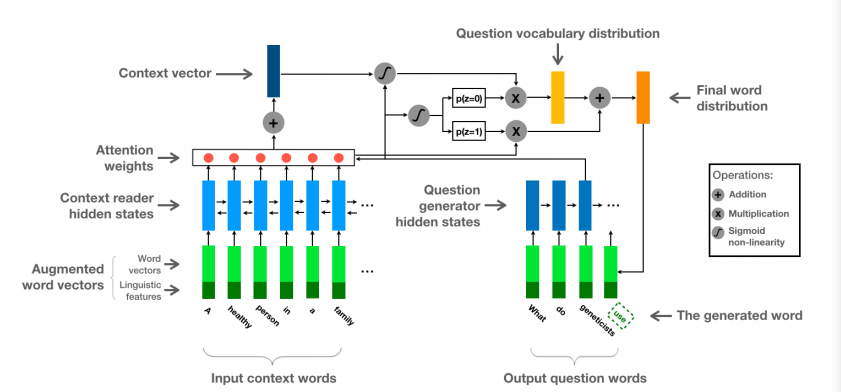
\includegraphics{img/qgnet.png}
\caption{ma}
\end{figure}

\begin{enumerate}
\def\labelenumi{\arabic{enumi}.}
\setcounter{enumi}{1}
\tightlist
\item
  In this paper
  \href{https://openreview.net/pdf?id=rk3pnae0b}{TOPIC-BASED QUESTION
  GENERATION}, they propose a topic-based question generation algorithm.
  The algorithm is able to take in a input sentence, a topic and a
  question type and generate a word sequence related to the topic,
  question type and the input sentence.
\end{enumerate}

They formulate a conditional likelihood objective function as mentioned
before to the model to learn.

Also, they go through a few general frameworks that have been employed
for solving the similar problem.

\begin{itemize}
\item
  The first one is \emph{seq2seq model} that uses a bidirectional LSTM
  as the encoder to encode a sentence and a LSTM RNN (Recurrent Neural
  Network) as the decoder to generate the target question.
\item
  The second approach is \emph{question pattern prediction and question
  topic selection algorithms}. It takes in an automatically selected
  phrase Q and fill this phrase into the pattern that was predicted from
  pre-mined patterns.
\item
  The last approach is \emph{multi-source seq2seq learning} which aims
  to integrate information from multiple sources to boost learning.
\end{itemize}

\begin{enumerate}
\def\labelenumi{\arabic{enumi}.}
\setcounter{enumi}{2}
\tightlist
\item
  In this paper \href{https://arxiv.org/pdf/1808.04961.pdf}{A Framework
  for Automatic Question Generation from Text using Deep Reinforcement
  Learning}, they implement a reinforcement learning(RF) framework that
  consists of a generator and an evaluator for this task.
\end{enumerate}

They refer to \emph{the generator} part of the model as the \(agent\)
and the \(action\) of the agent is to generate the next work in the
question. The probability of decoding a word is \[P_{\theta}(word)\]
with a stochastic policy.

\emph{The evaluator} part of the model will in turn assign a \(reward\)
for the output sequence predicted using the current \(policy\) by the
generator. Based on the reward assigned by the evaluator, the generator
updates and improves its current policy. In short, the goal in RL-based
question generation is to find a policy that can maximize the sum of the
\emph{expected return} at the end of the sequence generation.

\subsubsection{Summary}\label{summary}

In this QG section, we have discussed 3 different algorithms. Based on
our learning, we can conclude that a generative seq2seq model might be a
suggested model for this task. As for our objective function, we should
be foumulating a conditional probability distribution that is
conditioned on the provided content (i.e.~the video) and answers. As
suggested, we can use a bi-directional LSTM RNN as the encoder to encode
the content and use a LSTM RNN as the decoder to generate the question.

\subsection{Question Answering}\label{question-answering}

Now, let's move on to our question answering (QA) task. The general goal
of a QA model is to predict an answer to a question based on the
information found in the passage, given a passage and a question. By
solving this task, our system should be able to easily evaluate the
answer provided by learners and achieve the full automation of the
learning + feedback cycle.

Here are the overview of a basic QA model's implementation
{[}{\textbf{???}}{]}:

\begin{enumerate}
\def\labelenumi{\arabic{enumi}.}
\item
  Build representation for the passage and the question separately;
\item
  Incorporate the question information into the passage;
\item
  Get the final representation of the passage by directly matching it
  against itself;
\item
  Generate the answer.
\end{enumerate}

And the typical mechanims applied for solving such a problem include:

\begin{itemize}
\item
  Embedding
\item
  Encoder Decoder
\item
  Attention Mechanism
\end{itemize}

\subsubsection{Close-ended Questions}\label{close-ended-questions}

\paragraph{Visual Question Answering
(VQA)}\label{visual-question-answering-vqa}

VQA is a challenging research problem that focuses on providing a
natural language answer given any image and any free-form natural
language question. As we are managing to handle the video educational
content first, our problem will include both NLP and visual recognition
tasks. Therefore, VQA should be a great area to start with.

\subparagraph{Case Studies}\label{case-studies-1}

\begin{enumerate}
\def\labelenumi{\arabic{enumi}.}
\tightlist
\item
  In this paper
  \href{http://openaccess.thecvf.com/content_ECCV_2018/papers/Yalong_Bai_Deep_Attention_Neural_ECCV_2018_paper.pdf}{Deep
  Attention Neural Tensor Network for Visual Question Answering}, they
  propose a novel \emph{deep attention neural tensor network} that can
  discover the joint correlation over images, questions and answers with
  tensor-based representation.
\end{enumerate}

As for their workflow, they model one of the pairwise interaction
(i.e.~between image and question) by \textbf{bilinear features}, which
is further encoded with the third dimension (i.e.~answer) to be a
triplet using bilinear tensor product. During this step, the model takes
in a question + a corresponding image + candidate answers as the input.
A CNN (convolutional neural network) a GRU RNN are used for extracting
feature vectors and question respectively. Then the representation is
passed on as a \emph{multi-modal feature} and integrated by a
\textbf{bilinear pooling} module. Moreover, they decompose the
correlation of triplets by their question and answer types with a
\textbf{slice-wise attention module} on tensor to select the most
discriminative reasoning process inference.

In the end, they optimize the proposed network by learning a label
regression with KL-divergence losses. They claime that these techniques
enable them to do scalable training and fast convergence over a large
number of answer set. During the inference stage, they feed the
embeddings of all candidate answer into the network and then select the
answer which has the biggest triplet relevance score as the final
answer.

The high-level network architecture is as follows:

\begin{figure}
\centering
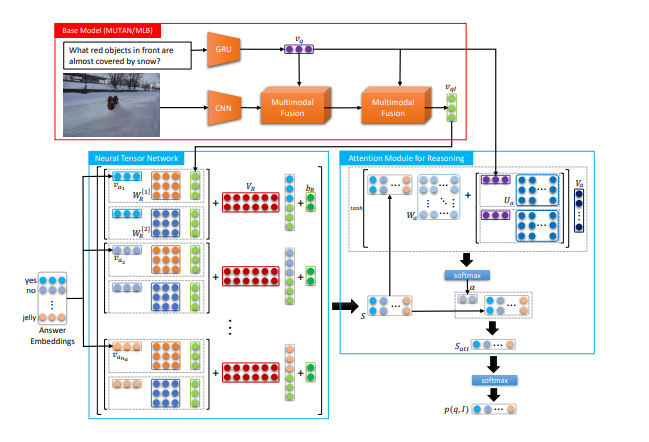
\includegraphics{img/vqa.png}
\caption{Deep Attention Neural Tensor Network}
\end{figure}

\begin{enumerate}
\def\labelenumi{\arabic{enumi}.}
\setcounter{enumi}{1}
\tightlist
\item
  In this paper \href{https://arxiv.org/pdf/1804.02088.pdf}{Question
  Type Guided Attention in Visual Question Answering}, they propose a
  model called \textbf{Question Type-guided Attention (QTA)}. This model
  utilizes the information of question type to dynamically balance
  visual features from both top-down and bottom-up orders.
\end{enumerate}

Also, they propose a \emph{multi-task extension} that is trained to
predict question types from the lexical inputs during training which
generalizes the network into applications that lack question type, with
a minimal performance loss.

As for their main contribution, they focus on developing an attention
mechanism that can exploit high-level semantic information on the
question type to guide the visual encoding process.

Specifically, they introduce a novel VQA architecture that can
dynamically gate the contribution of ResNet and Faster R-CNN features
based on the question type. In turn, it allows them to integrate the
information from multiple visual sources and obtain gains across all
question types.

\begin{enumerate}
\def\labelenumi{\arabic{enumi}.}
\setcounter{enumi}{2}
\tightlist
\item
  In this paper
  \href{https://www.ijcai.org/proceedings/2018/0513.pdf}{Multi-Turn
  Video Question Answering via Multi-Stream Hierarchical Attention
  Context Network}, they propose a hierarchical attention context
  network for context-aware question understanding by modeling the
  hierarchically sequential conversation context structure. They
  incorporate the multi-step reasoning process into \textbf{the
  multi-stream hierarchical attention context network} to enable the
  progressive joint representation learning of the multi-stream
  attentional video and context-aware question embedding.
\end{enumerate}

To construct their dataset, they collect the conversational video
question answering datasets from
\href{http://upplysingaoflun.ecn.purdue.edu/~yu239/}{YouTubeClips} and
\href{https://www.mpi-inf.mpg.de/departments/computer-vision-and-multimodal-computing/research/vision-and-language/tacos-multi-level-corpus/}{TACoS-MultiLevel}.
The first dataset has 1987 videos and the second dataset has 1303
videos. They invite 5 pairs of crowd-sourcing workers to construct 5
different conversational dialogs. In total, they have collected 37228
video question answering pairs for TACoS-MultiLevel data and 66806 ones
for YouTubeClips data.

\begin{enumerate}
\def\labelenumi{\arabic{enumi}.}
\setcounter{enumi}{3}
\tightlist
\item
  In this paper \href{https://arxiv.org/pdf/1512.02902.pdf}{MovieQA:
  Understanding Stories in Movies through Question-Answering}, they
  construct a new dataset ** MovieQA** dataset that can be used to
  evaluate automatic story comprehension from both video and text.
\end{enumerate}

They collect 408 subtitled movies and obtained their extended summaries
in the form of \textbf{plot synopses}(movie summaries that fans write
after watching the movie) from Wikipedia. They used plot synopses as a
proxy for the movie. They have annotators create both quizzes and
answers pairs by referring to the story plot. Time-stamp is also
attached with each question and answer pair.

In the second step of data collection, they used the multiple-choice
answers and question collected as the input to show to a different group
of annotators. By doing so, annotators could re-formulate the question
and answers for the sanity check.

\paragraph{Summary}\label{summary-1}

By going through the previous examples, we can see that VQA and few
similar algorithms introduced before are designed to efficiently process
image and text input data while making the inference based on the input.

Few main insights learned through the research. First, key components
for creating and trainnig a VQA model such as feature selection, feature
pooling and specifically designed attention mechanism. The input of the
mode is typically a video clip + question + answer pairs. A CNN and
sometimes a RNN is needed for such a task.

Another important learning is that we can follow the steps they take to
collect and annotate our training data by asking crowd-sourcing workers
to construct the question and answer pairs. Also, more advanced
algorithm like the one described above multi-stream hierarchical
attention context network is in need for dealing with video input data
in contrast to static pictures.

\paragraph{Dual Question-Answering
Model}\label{dual-question-answering-model}

Both Question Generaion(QG) and Question Answering(QA) are well-defined
2 sets of problems that aim to either infer a question or an answer
given the counterpart based on the context. However, they are usually
explored separately despite of their intrinsic complementary
relationship. In our case, a system needs to take on both roles
simultaneously.

Let's look into a few algorithms are designed for this.

\subparagraph{Case Studies}\label{case-studies-2}

1.In this paper \href{https://arxiv.org/pdf/1809.01997.pdf}{Dual
Ask-Answer Network for Machine Reading Comprehension}, they present a
model that can learn question answering and question generation
simultaneously. They tie the network components that playing the similar
roles into 2 tasks to transfer cross-task knowledge during training.

Then \emph{the cross-modal interaction} of question, context and answer
is captured with a pair of \textbf{symmetric hierarchical attention}
processes.

The high-level architecture of the model is illustrated as below:

\begin{figure}
\centering
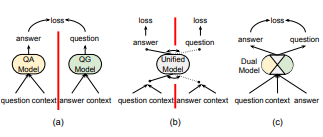
\includegraphics{img/qgqa.png}
\caption{Dual Ask-Answer Network 1}
\end{figure}

\begin{figure}
\centering
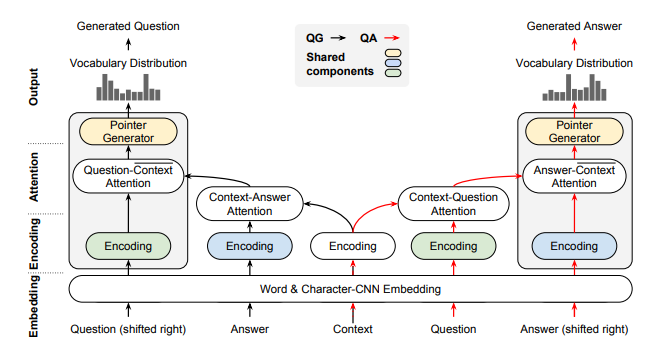
\includegraphics{img/daan.png}
\caption{Dual Ask-Answer Network 2}
\end{figure}

In short, the model is composed of the following components: embedding
layer, encoding layer, attention layer and output layer. The model is
fed with a question-context-answer triplet \((Q,C,A)\) and the decoded Q
and A from the output layer. Their loss function consists of 2 parts:

\begin{itemize}
\tightlist
\item
  negative log-likelihood loss
\item
  a coverage loss to penalize repetition of the generated text
\end{itemize}

\begin{enumerate}
\def\labelenumi{\arabic{enumi}.}
\setcounter{enumi}{1}
\tightlist
\item
  In this paper \href{https://arxiv.org/pdf/1805.05942.pdf}{Harvesting
  Paragraph-Level Question-Answer Pairs from Wikipedia}, they apply
  their question-answer pair generation system to 10000 top-ranking
  Wikipedia articles and create over a million question-answer pairs.
\end{enumerate}

In their task formulation part, they clarify that they break this task
into 2 sub-tasks:

\begin{itemize}
\tightlist
\item
  candidate answer extraction
\item
  answer-specific question generation
\end{itemize}

To complete the tasks, they first identify a set of question-worthy
candidate answer set \(ans = (A1, A2,...Ai)\). For each candidate answer
\(A_i\), they then aim to generate a question \(Q\) -a sequence of
tokens \({y1,y2,...yn}\) - based on the sentence S that contains
candidate \(A_i\) such that - Q asks about an aspect of \(A_i\) (of
potential interest to a human) - Q might rely on information from
sentences that precedes S in the paragraph. Mathematically, they compose
a function \[Q = argmax_Q P(Q|S,C)\].

\begin{enumerate}
\def\labelenumi{\arabic{enumi}.}
\setcounter{enumi}{2}
\tightlist
\item
  In this paper
  \href{http://cvboy.com/pdf/publications/cvpr2018_iqan.pdf}{Visual
  Question Generation as Dual Task of Visual Question Answering}, they
  propose an end-to-end unified model, \textbf{Invertible Question
  Answering (iQAN)} to introduce question generation as a dual task of
  question answering to improve VQA performance.
\end{enumerate}

In achieving their goal, they leverage the \textbf{dual learning}
framework that is proposed in machine translation area initially, which
uses \(A-to-B\) and \(B-to-A\) translation models to form two closed
translation loops and let them teach each other through a
\emph{reinforcement learning process}.

In their VQA component, given a question \(q\), an RNN is used for
obtaining the embedded feature \textbf{q}, and CNN is used to transform
the input image \(v\) into a feature map. A \emph{MUTAN-based attention
module} is then used to generate a question-aware visual feature \(v_q\)
from the image and the question. Later, another \emph{MUTAN fusion
module} is used for obtaining the answer feature \(a\hat{}\)

\begin{enumerate}
\def\labelenumi{\arabic{enumi}.}
\setcounter{enumi}{3}
\tightlist
\item
  In this paper \href{https://arxiv.org/pdf/1709.01058.pdf}{A Unified
  Query-based Generative Model for Question Generation and Question
  Answering}, they propose a query-based generative model for solving
  both tasks. The model follows the classic \emph{encoder-decoder}
  framework. The \textbf{multi-perspective matching encoder} that they
  are implementing is a bi-directional LSTM RNN model that takes a
  passage and a query as input and perform query understanding by
  matching it with the passage from multiple perspectives;
\end{enumerate}

The decoder is an \textbf{attention-based LSTM RNN} model with
\emph{copy and coverage} mechanism. In the QG task, a question will be
generated from the model given the passage and the target answer;
whereas in the QA task, the answer will be generated given the question
and the passage.

They also leverage a \emph{policy-gradient reinforcement learning}
algorithm to overcome \emph{exposure bias} (a major problem resulted
from sequence learning with cross-entropy loss function).

They case both QG and QA tasks into one process by firstly matching the
input passage against the query, then generating the output based on the
matching results.

As for the training, they first pretrain the model with cross-entropy
loss and then they fine tune the model parameters with policy-gradient
reinforcement learning to alleviate the exposure bias problem. They end
up adopting a similar sampling strategy as the scheduled sampling
strategy for generating the sampled output during the reinforcement
learning process.

\paragraph{Summary}\label{summary-2}

As mentioned earlier, QG and QA tasks are intrinsically bounded and one
cannot find solution for either of them without taking the other party
into account.

In this section, we have discussed some approaches that many groups of
people have taken to help machine operate on both tasks simultaneously.
Some exciting findings have been presented here.

For our problem, it is very motivating to see these progress and learn
from their approaches. In sum, our general setup is similar to dual
learning framework, we need to tie QG and QA part of the algorithms
together. In the first diagram of the section, we can see that they
connect the loss function from both sides of the model and it is very
similar to the strategy adopted by
\href{https://en.wikipedia.org/wiki/Generative_adversarial_network}{GAN}
(Generative adversarial network). Some advanced mechanisms are proposed
as well for effectively solving these tasks i.e.~symmetric hierarchical
attention and policy-gradient reinforcement learning algorithm.

\subsubsection{Open-ended Question}\label{open-ended-question}

\paragraph{Problem Formulation}\label{problem-formulation-1}

\begin{quote}
Open-ended questions bring clarity.
\end{quote}

As we mentioned above, the open-ended question could be roughly split
into 2 categories. A general open-ended question or a specific
open-ended question.

Technically specking, these 2 categories are not that particular
distinct since both problems require the system to draw some conclusion
based on the context and question provided; As for the answer, it is
allowed to have a pretty high degree of freedom. Therefore, our system
should be able to evaluate the answer with relatively flexible rules or
standards.

Based our assumptions, we will combine these 2 problems into 1 for now
for our further investigation.

It may appear unapproachable at the first glance to teach a system to
have answers for or evaluate this type of problems. Again, we need to
reframe our problem and then break it apart.

Based on our research, we believe it is helpful to think of this type of
issue as a particular type of QA problem; the difference is that after
the QA procedure, we need to match and evaluate the answers generated by
machine and the learner such that we can provide an adequate evaluation.

Let's start by looking at an existing knowledge evaluation system that
has been used for grading the essays automatically - \textbf{Automated
essay scoring (AES)}. AES focuses on automatically analyzing the quality
and assigning a score of a piece of writing . AES systems could rely not
only on grammars, but also on more complex features such as semantics,
discourse and pragmatics. It has four general types:

\begin{itemize}
\item
  Essay Grade: it is known as the first AES system.
\item
  Intelligent Essay Assessor: it is using Latent Semantic Analysis
  features
\item
  E-rater: it has been used by the ETS to score essay portion of GMAT
\item
  IntelliMetric: it is developed and used by the College Board for
  placement purposes.
\end{itemize}

Below are some research findings we consider as useful for our unified
goal.

\subparagraph{Case Studies}\label{case-studies-3}

\begin{enumerate}
\def\labelenumi{\arabic{enumi}.}
\tightlist
\item
  In this paper \href{http://aclweb.org/anthology/N18-1024}{Neural
  Automated Essay Scoring and Coherence Modeling for Adversarially
  Crafted Input}, they develop a network that can effectively learn
  connectedness features between sentences and propose a framework for
  integrating and jointly training the local coherence model with a
  state-of-art AES.
\end{enumerate}

They examine the robustness of the AES model on adversarially crafted
input and specifically focus on input related to local coherence; A
local coherence model can evaluate the writing based on its ability to
rank coherently ordered sequence of sentences higher than their
counterparts.

The models they used are \emph{Local Coherence (LC)} model and LSTM AES
model. The first model has 2 main parts: sentence representation and
clique representation; and he second model is a combined model that does
vector concatenation and joint learning.

\begin{enumerate}
\def\labelenumi{\arabic{enumi}.}
\setcounter{enumi}{1}
\tightlist
\item
  In this paper
  \href{https://www.ijcai.org/proceedings/2018/0512.pdf}{Open-Ended
  Long-form Video Question Answering via Adaptive Hierarchical
  Reinforced Networks}, they study the problem of open-ended video
  question answering from the viewpoint of the \emph{adaptive
  hierarchical reinforced encoder-decoder network} learning.
\end{enumerate}

They present the adaptive hierarchical encoder network to learn the
joint representation of the long-form video contents according to the
question with adaptive video segmentation. They also develop the
reinforced decoder network to generate the neural language answer for
open-ended video question answering. Meanwhile, they construct a
large-scale dataset for open-ended long-form video QA and validate the
effectiveness of the proposed method.

The framework of \textbf{Adaptive Hierarchical Reinforced Networks} is
are below:

\begin{figure}
\centering
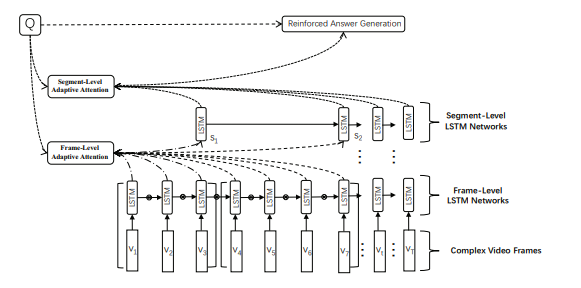
\includegraphics{img/oe.png}
\caption{Open-Ended Long-form Video QA Network}
\end{figure}

The first part of the model is the hierarchical encoder networks that
learn the joint representation of multimodal attentional video and
textual question with adaptive video segmentation.

The second part is the reinforced decoder networks that generate the
natural language answers for open-ended video question answering.

\begin{enumerate}
\def\labelenumi{\arabic{enumi}.}
\setcounter{enumi}{2}
\tightlist
\item
  In this paper, \href{https://arxiv.org/pdf/1805.11752.pdf}{Multi-turn
  Dialogue Response Generation in an Adversarial Learning Framework},
  they propose an adversarial learning approach that can generate
  multi-turn dialogue responses. The network framework that they
  introduce is call \emph{hredGAN} that is based on \emph{conditional
  GANs}. The generator part of the model is a modified
  \textbf{hierarchical recurrent encoder-decoder network (HRED)} and the
  discriminator is a word-level bi-directional LSTM RNN that shares
  context and word embedding with the generator.
\end{enumerate}

During the inference step, \emph{noise sampling} is conditioned on the
dialogue history and is used to perturb the generator's latent space for
generating possible responses. The final response is the one ranked the
best by the discriminator.

In sum, their hredGAN combines both generative and retrieval-based
multi-turn dialogue systems to improve the model's performance. One of
the special design of the model is that the generator and the
discriminator share the context and word embedding and this allows for
joint end-to-end training using back-propagation.

\subparagraph{Summary}\label{summary-3}

Based on our limited research, we found that it is achievable for our
system to generate the answers for open-ended questions based on the
educational video and provide appropriate feedback/rating based on the
current techniques. The first paper presents a newly developed AES model
that can rate learner's writing by taking into account some special
standand. It also demonstrates a possible way of enhance the AES model
by training it with the adversarially crafted input.

In the second paper, we discuss a network that can answer the open-ended
questions based on the video and a given question. Their Adaptive
Hierarchical Reinforced Networks are composed of hierarchical encoder
networks and the reinforced decoder networks. It is possible for us to
adopt their general framework trained with our educational video data
specifically.

Similar to the second paper, the last paper shows that it is possible to
generate responses conditioned on the context. By leveraging conditional
GAN model framework, their model's performance is significantly
improved.

\subsection{Summary of Learning and Feedback
Networks}\label{summary-of-learning-and-feedback-networks}

Based on our previous discussion, we find that both QG and QA (including
VQA) tasks have been well-studied. A number of specifically designed
algorithms were presented and proved effective for solving these
problems.

There is also plenty of research has also been done in open-ended
question answering realm. Though the performance may not be gauranteed,
some techniques presented above are greatly relevant and thought
provoking such as AES model and open-ended question answering networks.

Current research is promising but we need more research and innovation
in this area.

However, we are confident that by combining some techniques introduced
before to create such a coherent EC2QA network is not that far-fetched.

\subsubsection{Datasets and Annotation
Needed}\label{datasets-and-annotation-needed}

In order to approach this problem from scratch, we need to create our
own dataset for which we will provide some related resources to start
with:

\begin{enumerate}
\def\labelenumi{\arabic{enumi}.}
\tightlist
\item
  \href{https://research.google.com/youtube8m/}{YouTube-8M Dataset}.
  This is a large-scale labeled video dataset that consists of millions
  of YouTube video IDs, with high-quality generated annotations from a
  diverse vocabulary of 3800+ visual entities. As you can see from its
  introduction, it comes with precomputed audio-visual features from
  billions of frames and audio segments. In short, we can expect the
  following content from this dataset:
\end{enumerate}

\begin{itemize}
\item
  the dataset consists of 6.1M videos URLs, labeled with a vocabulary of
  3863 visual entities
\item
  the video-level dataset comes out to be 18 GB in size, while the
  frame-level features are approximately 1.3 TB
\item
  it comes with pre-extracted audio \& visual features from every second
  of video.
\end{itemize}

Though the video content is not limited to education category, we can
still use it to get a strong baseline model.

Naturally, the next step would be constrain our model to train on
particularly educational content. The data needed for training may
include the raw video clip, annotation/caption of the whole video
content, and audio part of the video.

\begin{enumerate}
\def\labelenumi{\arabic{enumi}.}
\setcounter{enumi}{1}
\tightlist
\item
  In this study
  \href{http://jofdl.nz/index.php/JOFDL/article/download/255/198}{Video
  Captions for Online Courses: Do YouTube's Auto-generated Captions Meet
  Deaf Students' Needs?}, they studied auto-generated captions generated
  on YouTube online courses. They find that, on average, there were 7.7
  phrase errors per minute of a total 68 minutes video caption. We still
  need to do a lot of annotation work before we can finally compose our
  own training dataset.
\end{enumerate}

Other resources that could possibly help us with out tasks are as below:

\begin{enumerate}
\def\labelenumi{\arabic{enumi}.}
\setcounter{enumi}{2}
\tightlist
\item
  \href{http://videomcc.org/}{VideoMCC}. In their paper, they formulate
  Video Multiple Choice Caption (VideoMCC) as a way to assess video
  comprehension through an easy-to-interpret performance measure. In
  their paper \href{https://arxiv.org/pdf/1606.07373.pdf}{VideoMCC: a
  New Benchmark for Video Comprehension} they propose to cast video
  understanding in the form of multiple choice tests that assess the
  ability of the algorithm to comprehend the semantics of the video.
  Example is as below:
\end{enumerate}

\begin{figure}
\centering
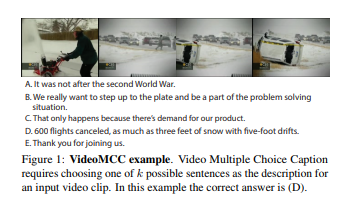
\includegraphics{img/mcc.png}
\caption{VideoMCC}
\end{figure}

\begin{enumerate}
\def\labelenumi{\arabic{enumi}.}
\setcounter{enumi}{3}
\tightlist
\item
  As what we have covered earlier, this paper
  \href{https://arxiv.org/pdf/1512.02902.pdf}{MovieQA: Understanding
  Stories in Movies through Question-Answering}, they introduced a new
  dataset called MovieQA dataset that can evaluate automatic story
  comprehension from both video and text.
\end{enumerate}

Here are 2 figures that can help you better understand their dataset:

\begin{figure}
\centering
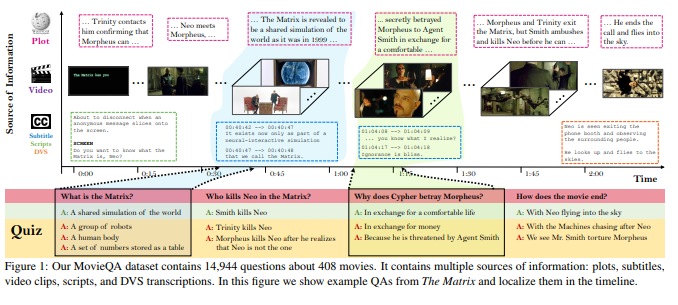
\includegraphics{img/movieqa1.png}
\caption{MovieQA\_1}
\end{figure}

\begin{figure}
\centering
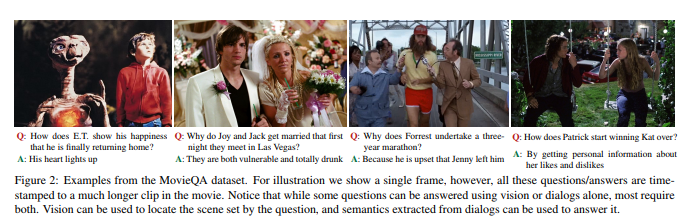
\includegraphics{img/movieqa2.png}
\caption{MovieQA\_2}
\end{figure}

\begin{enumerate}
\def\labelenumi{\arabic{enumi}.}
\setcounter{enumi}{4}
\item
  In this paper \href{https://arxiv.org/pdf/1806.00186.pdf}{Video
  Description: A Survey of Methods, Datasets and Evaluation Metrics}
  multiple methods, datasets and evaluation metrics for video
  description task in a comprehensive survey.
\item
  Inspired by this paper
  \href{https://arxiv.org/pdf/1808.07036.pdf}{QuAC : Question Answering
  in Context} in which they present QuAC dataset for QA in Context that
  contains 14K information-seeking QA dialogs such as a student who
  poses a sequence of freeform question to learn as much as possible
  about a hidden Wikipedia text or a teacher who answers the questions
  by providing short excerpts from the text, we are convinced that it is
  might also be possible to develop a system that can allow student to
  pause the video and ask our system a information-seeking question and
  then get the answer from our system based on the current content. .
\end{enumerate}

\section{Knowledge Graph}\label{knowledge-graph}

Next, we need to consider how we can select an adequate and relevant
learning material and generate an effective learning map for the
learners based on their current progress and the general knowledge
graph/map, given the ever growing amount of educational content on the
web.

As I mentioned earlier, learning is a knowledge accumulation process.
Knowledge itself has its unique structure that can help us learn in a
most effective and productive way. Knowledge Graph is a great tool that
we developed to map and present the structure of knowledge. In shirt,
knowledge graphs are collections of relational facts, where each fact
states that a certain relation holds between 2 entities.

Now we will consider the knowledge graph as the backbone.

\subsection{What is a graph?}\label{what-is-a-graph}

\begin{quote}
Graphs are networks of dots and lines - Graph Theory (Dover Books)
\end{quote}

Mathematically speaking, graphs are mathematical structures used to
model pairwise relations between objects. A graph in this context is
made of vertices, nodes, or points which are connected by edges, arcs or
lines. Typically a graph consists of two sets. A set of vertexes and a
set of edges \[GRAPH_{v,e} =
 \begin{pmatrix}
  v_{1,1} & a_{1,2} & \cdots & a_{1,n} \\
  e_{2,1} & e_{2,2} & \cdots & e_{2,n} \\
 \end{pmatrix}\]

As for the knowledge graph, it is a graph representation of a knowledge
base. Often when people talk about a knowledge graph, they are referring
to the multi-relational graph used by Google and its services to enhance
search engine's results with information gathered from a variety of
sources. Per Wikipedia,
\href{https://developers.google.com/knowledge-graph/\#knowledge_graph_entities}{Google's
Knowledge Graph} uses a graph database to provide structured and
detailed information about the topic in addition to a list of links to
other sites.

In general, a knowledge graph represents a knowledge domain. It connects
things of different types in a systematic way. Knowledge graphs encode
knowledge arranged in a network of nodes and links rather than tables
and columns. With knowledge graphs, people and machines can benefit from
a dynamically growing semantic network of facts about things. In other
words, we can use it to capture the facts related to people, processes,
applications, data and many other custom objects as well as their
relationships among them.

Also, we have found a lot of applications that demonstrate that existing
generic knowledge graphs have shown advantages to support semantic
search(i.e.~Google's Knowledge Graph), personal assistant(i.e.~Apple's
Siri) and deep question answering (i.e.~Wolfram Alpha and IBM's Watson).

\subsection{Problem Formulation}\label{problem-formulation-2}

Given we've implemented the learning and feedback module, knowing where
a given piece of education content fits into the knowledge space is a
vital task if we want the knowledge footprint to make a learner
predictable to others as well as being able to recommend new educational
content that the learner can take on successfully. We will need the
following things to connect educational content.

\begin{quote}
A classifier to take a piece of educational content
\end{quote}

A graph dedicated to education should do the following:

\begin{itemize}
\item
  Provide flexibility to add new subjects
\item
  Connect related subjects to each
\item
  Map concepts with the subject
\item
  Connect concepts related to the content
\end{itemize}

\begin{figure}
\centering
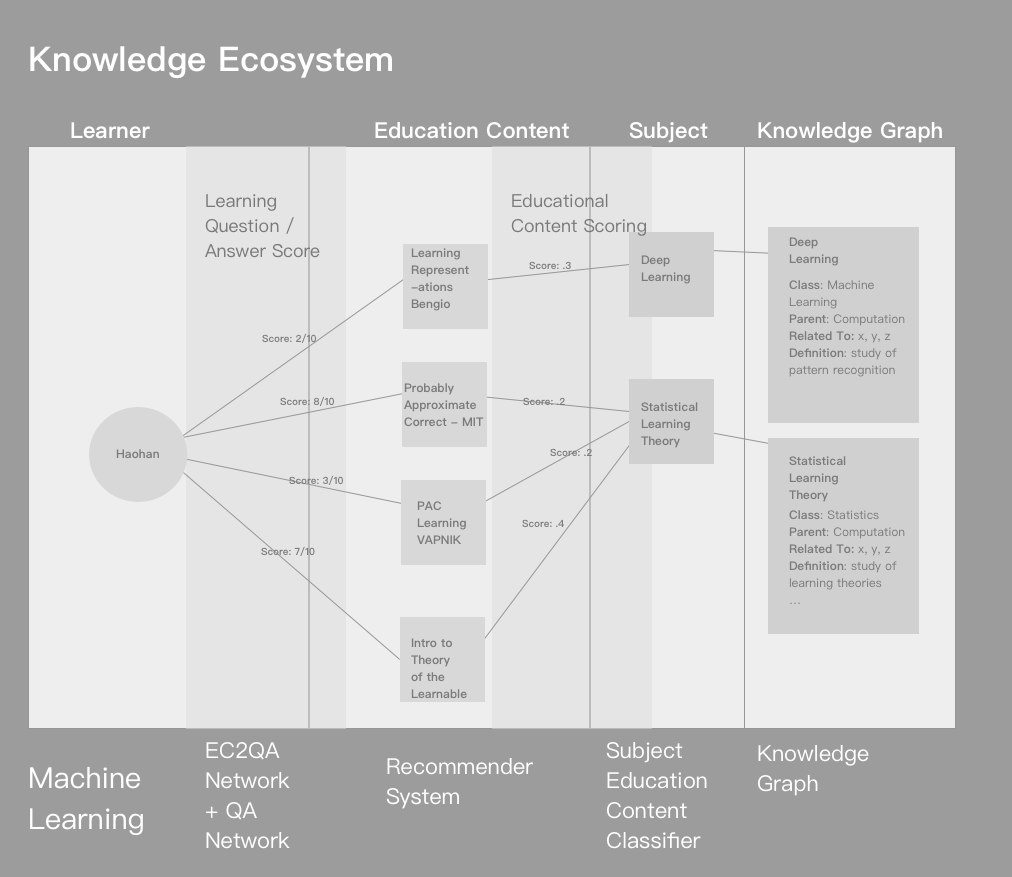
\includegraphics{img/knowledgeEcosystem.png}
\caption{Knowledge Ecosystem}
\end{figure}

\subsection{Automatic Knowledge Graph
Construction}\label{automatic-knowledge-graph-construction}

Classic knowledge representation techniques allow a knowledge engineer
to create rules that can be interpreted by a reasoner to infer new or
missing triples(subject, predicate, object). These rules are usually
expressed through an ontology which allows for the propagation of
properties from top classes to the lower classes.

However, we are looking for solutions that can allow us to complete our
educational knowledge graph construction process. Based on our research,
generic knowledge graphs usually cannot sufficiently support many
domain-specific applications i.e.~education and finding the
representation of the graph to feed the triples into a machine learning
algorithm is still an open area of research. As a start, let's focus on
how to automate the education knowledge graph construction process.

There have been several papers that provide promising results to the
automation of constructing a knowledge graph. Let's take a look.

\subsection{Case Studies}\label{case-studies-4}

\begin{enumerate}
\def\labelenumi{\arabic{enumi}.}
\tightlist
\item
  In this paper
  \href{https://ieeexplore.ieee.org/document/8362657}{KnowEdu: A System
  to Construct Knowledge Graph for Education}, the authors propose a
  system, titled KnowEdu, that can automatically construct a knowledge
  graph for education. In short, the system is able to extract concepts
  of subjects or courses and then identifies the educational relations
  between the concepts.
\end{enumerate}

More importantly, it adopts the neural sequence labeling algorithm on
pedagogical data to extract instruction concepts. They then employ
probabilistic association rule mining on learning assessment data to
identify the significance of each of the relations.

In sum, their system consists of the following modules:

\begin{itemize}
\item
  Instructional Concept Extraction Module to extract instructional
  concepts for a given subject or course.
\item
  Educational Relation Identification Module to identify the educational
  relations that interlink instructional concepts to assist the learning
  and teaching process directly.
\end{itemize}

Below is a block diagram of KnowEdu System.

\begin{figure}
\centering
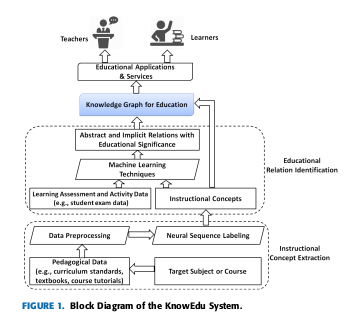
\includegraphics{img/knowedu.png}
\caption{knowedu}
\end{figure}

They used conditional random field (CRF) model for entity or terminology
recognition task. Moreover, they adopt neural network, or more
particularly Gated recurrent unit network (GRU) architecture for neural
sequence labeling on educational entity extraction task.

In terms of relation identification they implement probabilistic
association data mining techniques on learning assessment adata and
accomplish the task of educational relation identification.

A snapshot of the knowledge graph for mathematics generated by knowedu
system.

\begin{figure}
\centering
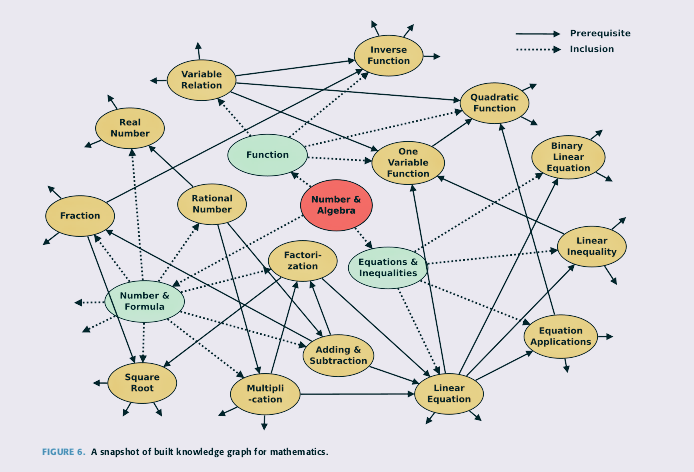
\includegraphics{img/kg.png}
\caption{knowledge\_graph}
\end{figure}

Below are some approaches related to knowledge graph (KG) embedding
which is used to embed components of a KG including entities and
relations into continuous vector space so as to simply the manipulation
while preserving the inherent structure of a KG.

As for its benefits and importance for our task, it can help with a
variety of downstream tasks i.e.~KG completion and relation extraction,
and hence be used to drastically improve the information acquisition
speed for KG.

\begin{enumerate}
\def\labelenumi{\arabic{enumi}.}
\setcounter{enumi}{1}
\tightlist
\item
  In this paper
  \href{http://www.mlgworkshop.org/2018/papers/MLG2018_paper_5.pdf}{Generalized
  Embedding Model for Knowledge Graph Mining}, they have presented a
  model for learning neural presentation of generalized knowledge graphs
  using a novel multi-shot unsupervised neural network model, called the
  \textbf{Graph Embedding Network (GEN)}. This model is able to learn
  different types of knowlege graphs from a universal perspective and it
  provides flexibility in learning representations that work on graphs
  conforming to different domains.
\end{enumerate}

In developing their model, they extend the traditional one-shot
supervised learning mechanism by introducing a multi-shot unsupervised
learning framework where a 2-layer MLP network for every shot. This
framework can in turn be used to accommodate both homogeneous and
heterogeneous networks.

\begin{enumerate}
\def\labelenumi{\arabic{enumi}.}
\setcounter{enumi}{2}
\tightlist
\item
  In this paper
  \href{https://openreview.net/pdf?id=rJ4qXnCqFX}{Probabilistic
  Knowledge Graph Embeddings}, they explored a new type of embedding
  model that can link prediction in relational knowledge graph. They
  start from a problem that even large knowledge graphs typically
  contain only few facts per entity, leading effectively to a small data
  problem where parameter uncertainty matters. As for the solution, they
  suggest that the knowledge graphs should be treated within a Bayesian
  framework.
\end{enumerate}

In short, they present a probabilistic interpretation of existing
knowledge graph embedding models. By reformulating the models like
ComplEx and DistMult, they construct the generative models for
relational facts.

They also apply stochastic variational inference to estimate an
approximate posterior for each entity and relation embedding in the
knowledge graph. By doing so, they can estimate the uncertainty, but
more importantly, they can use gradient-based hyperparameter
optimization by stochastic gradient descent on the optimized variational
bound.

As a result, their model shows experimentally new state-of-art results
in link prediction task.

\subsection{Summary of Knowledge
Graph}\label{summary-of-knowledge-graph}

Based on our research, there has been much progress in automated
knowledge graph construction applied to the education domain using deep
learning and other machine learning techniques.

The first paper introduces a system that almost exactly matches our
goal. The authors carefully walk us through the current progress and
possible solutions for solving each of the obstacles in developing a
education based knowledge graph. For the instructional concept
extraction task, they use both CRF model and neural sequence labeling
algorithm to achieve high performance. They employ probabilistic
association rule mining on learning assessment data to identify the
relations with educational significance.

The last 2 papers demonstrate the progress that has been made in KG
embedding learning domain. As mentioned above, as one of the most
effective methods in representing knowledge graphs.

\subsubsection{Key Components}\label{key-components}

Here are some key components that we found important of building an
automated knowledge graph for education:

\begin{enumerate}
\def\labelenumi{\arabic{enumi}.}
\item
  Entity recognition that aims to extract concept of interest from
  structured or unstructured data.
\item
  Relation identification that leverages on the semantic meaning of
  data.
\end{enumerate}

\subsubsection{Possible Next Steps}\label{possible-next-steps}

Here are some of our research summary regarding the steps of creating
such an educational knowledge graph:

\begin{enumerate}
\def\labelenumi{\arabic{enumi}.}
\item
  In terms of entity recognition task, We need to first get the data
  from some reliable open semantic sources i.e.~Wikipedia or Freebase.
  Or we can crawl the data online on our own to find high quality
  training data. In the next section we will be listing out some
  resources that might help.
\item
  Next, we need to create the model to map the relation among the
  entities. There are plenty of great github that we can use to help us
  with this task. Or we can use some tools developed for this purpose
  i.e.~node.js and Wolfram Mathematica embedded symbolic functions or
  just TensorFlow. The typically techniques we will employ are NLP and
  semantic data tagging or labeling techniques.
\item
  Naturally, after the entity extraction and relationship mapping we
  will visualize our map.
\end{enumerate}

\subsubsection{Datasets and Annotation Needed
needed}\label{datasets-and-annotation-needed-needed}

\begin{enumerate}
\def\labelenumi{\arabic{enumi}.}
\tightlist
\item
  \href{https://ai.google/research/pubs/pub45634}{Knowledge Vault}: A
  web-scale approach to probabilistic knowledge fusion. In this paper
  \href{https://dejanseo.com.au/wp-content/uploads/2014/08/Knowledge-Vault-A-Web-Scale-Approach-to-Probabilistic-Knowledge-Fusion.pdf}{Knowledge
  Vault: A Web-Scale Approach to Probabilistic Knowledge Fusion}, they
  introduce Knowledge Vault that combines extraction from Web content
  (obtained through analysis of text, tabular data, page structure, and
  human annotation) with prior knowledge derived from existing knowledge
  repositories.
\end{enumerate}

They employ a supervised machine learning models for fusing these
distinct information sources. As a result, their system can
automatically construct a web-scale probabilistic knowledge base.

\begin{enumerate}
\def\labelenumi{\arabic{enumi}.}
\setcounter{enumi}{1}
\tightlist
\item
  \href{https://developers.google.com/knowledge-graph/\#knowledge_graph_entities}{Google
  Knowledge graph Search API}.
\end{enumerate}

Below are some resources that might be helpful for starting such a job
from scratch:

\begin{enumerate}
\def\labelenumi{\arabic{enumi}.}
\setcounter{enumi}{2}
\item
  \href{https://developers.google.com/search/docs/guides/intro-structured-data}{Understand
  how structured data works} by Google.
\item
  \href{wikipedia.com}{Wikipedia}
\item
  \href{Freebase.com}{Freebase}
\end{enumerate}

\section{Knowledge Journeys}\label{knowledge-journeys-1}

The collective knowledge graph is our `ground truth' that can be used to
serve every learner in the ecosystem and be applied universally to some
extent, but everyone's learning journey is still unique to the learner.
Everyone seems to have their unique set of problems that they are
curious about and they will end up taking on their own journey towards
the mastery. As a result, their knowledge journeys will need several
degrees of freedom to represent learner's history, interests, and whom
they are similar to.

We cannot possibly put such an online educational ecosystem into use
without taking this crucial factor into our account.

Let's first formulate our problem. Below are few key components of such
a task:

\begin{enumerate}
\def\labelenumi{\arabic{enumi}.}
\item
  First, we need to have a system that can match all the content that a
  learner has acquired with the collective educational knowledge graph;
\item
  Generate their personal knowledge graph with the timestamps on each
  content and the subject(s) it belongs to;
\item
  Unfold the timestamps and map the previous generated static knowledge
  graph onto a timeline that can display a learner's knowledge as a
  personal knowledge acquisition storyline/gallery;
\item
  Adaptively update the journey along with a learner's learning
  progress.
\end{enumerate}

As the outcome, a learner's knowledge journey will be available anytime
for the learner to review the content that he/she has learned at any
past moment and for others to look into the details of one's journey.

\section{Knowledge Footprint}\label{knowledge-footprint-1}

Just a quick review of this concept we introduced earlier, knowledge
footprint is going to be presented as a badge or a symbol to represent
someone's knowledge state at a fix point in time. In a sense, this
thumbnail view of a learner's knowledge will evolve and change when a
learner continues his/her learning journey. By constructing such
symbol(s), a learn can easily understand their current knowledge states
relatively to their past and others and timely make an adjustment to
alter their future learning plan.

In terms of the techniques that can be applied for this task, we would
primarily consider unsupervised learning and dimensionality reduction
algorithms to help us uncover and represent the visible and invisible
dimensions of a learner's knowledge journey and state. Also, we believe
it is going to be a teamwork that requires people like machine learning
and deep learning researchers, educators, and designers to work
collaboratively to ensure the optimal outcome.

Note that we will not discuss the detailed research findings or
implementation steps of the last 2 elements in this essay. We will leave
these areas for our future research.

\subsection{Possible Next Steps}\label{possible-next-steps-1}

As a reasonable next step, we would also like our system to be as
personalized as possible so as to provide guidance for a learner along
their knowledge journey, given that our system has already encoded and
possessed the information of a learner's footprint and journey.

In this case, a recommender system might be a desirable choice for
handling such a job since it is an intuitive line of defense against
consumer over-choice given the ever growing educational content
available on the web.

\chapter{Next Steps}\label{next-steps}

\section{Overview}\label{overview}

We have now proposed one approach to better represent a modern
individual's knowledge by taking the world of unstructured educational
content (Youtube videos, Medium articles, etc), classifying it by it's
concepts which belong to one or more subjects from a education-based
knowledge graph. We've introduced learning and feedback by testing a
learner's knowledge by generating a set of questions and answers
conditioned on an educational content without the need for the educator
to include questions and answers.

We surveyed some of the relevant machine and deep learning research,
proposed the Educational Content to Questions and Answers (EC2QA)
network, a novel neural network for taking in any type of educational
content and generating a set of questions, answers, and evaluation of a
learner's knowledge understanding.

We then proposed to tie these components together as an adaptive
knowledge ecosystem consisting of an individual's knowledge footprint,
mapped to a central knowledge graph, visualised over time as a learner's
knowledge journey. This would serve to enable the independent (aspiring
or current) learner to pursue their life-long self-study. It would take
into consideration the education they acquired from unstructured
sources, thereby formalising their informal knowledge for themselves and
others.

\section{Challenges}\label{challenges}

There will be many challenges in coming up with solutions to enable
knowledge acquisition and representation at the learner and group level.
We will address some of the primary challenges to designing the
components of the proposed knowledge ecosystem:

\begin{itemize}
\tightlist
\item
  Datasets -- EC2QA dataset -- Knowledge graph dataset
\item
  Deep Learning Architecture -- EC2QA network
\end{itemize}

For our purposes we will focus on the EC2QA network and dataset as the
main focus for our next steps.

\section{EC2QA dataset}\label{ec2qa-dataset}

The success of deep learning techniques are predicated on the assumption
that one needs a significant amount of data to train a large neural
network to learn the representation that captures the set of admissible
functions needed to learn a given set of concepts.

The EC2QA network will also face the same challenges it requires a large
dataset of educational content (i.e.~Youtube videos, Wikipedia pages or
Medium articles) along with a set of questions, which will have a set of
correct and incorrect answers for each question.

\[
 \{content1: \{question1: \{answer1, answer2,...\},  question2: \{answer1, answer2,...\},...\},...
\]

\begin{longtable}[]{@{}llll@{}}
\toprule
Educational Content & Concepts & Subjects & Questions and Answer
Pairs\tabularnewline
\midrule
\endhead
Robert Sapolsky Human Behavioral Biology Lecture 1:
{[}{[}{[}0,23,435\ldots{}\ldots{}{]}{]}{]} & neurobiology, neurological
disease, gene, nature vs nuture, hormones & Neurobiology, Biology,
Neuroscience, Behavioral Science & \{ ``What is the definition of human
behavioral biology ``: correct\_answer: ``'', in\_answer:
``\}\tabularnewline
\bottomrule
\end{longtable}

There are many approaches to decreasing the amount of data needed while
still learning a good representation of the set of concepts the
architecture needs to learn. We will present an approach that we believe
best utilises the intrinsic structure of educational content and using
the minimal amount of data.

\begin{enumerate}
\def\labelenumi{\arabic{enumi}.}
\item
  The network can be trained on unstructured educational content without
  questions or answers to create an \emph{education embedding} by
  leveraging unsupervised techniques like variational auto-encoder
  (VAE). This requires a dataset of educational content, possibly many
  media types(audio/video/text). This could also be done by using a
  semi-supervised technique by supervising the media type and learning
  representations for the types of educational content.
\item
  The network can then be trained on \textbf{existing} educational
  content that \emph{already} has preexisting questions and answers for
  specific parts of the content (i.e.~Khan Academy, Udacity, Coursera).
  The domain of structured educational content is surely very different
  from the unstructured content and may hinder the network but we
  believe it might be the case that it helps more than it hinders but we
  cannot guarantee this so it is worth experimenting.
\item
  The final step is annotating a set of unstructured educational content
  with questions and answers.
\end{enumerate}

\section{Education Partners}\label{education-partners}

The second step above requires a large amount of existing educational
content paired with existing questions and answers. This data is rich
and informative; it could help us learn an early representation and use
less of our original dataset (\#3) for learning such a representations.
Most of these datasets have been created by experts and educators and
their efforts could be valuable for our model to learn from. For this
purpose, we would need to partner with large (in terms of library of
content) educational institutions (i.e.~Udacity, Coursera, MOOCs, Edx,
Khan Academy) to work with their datasets for pretraining and
collaborate on how we annotate the space of unstructured educational
content.

\section{Educator Enrichment}\label{educator-enrichment}

The third and final dataset that would be used as our primary data
source to train and test the model's performance, remains the most
important component as well as being the most time and labour intensive.
Partnering with educators and subject matter experts to source the
subspace of unstructured educational content and to create questions and
answers, we would eventually arrive at a curated dataset that our model
would be primarily trained on. The end result would be a new benchmark
that other researchers can begin to build newer architectures to make
progress on the problem domain.

\section{Minimum Viable Dataset
(Benchmark)}\label{minimum-viable-dataset-benchmark}

We propose to narrow the problem space and jumpstart research in this
area by focusing on only one subject (i.e.~psychology, mathematics, or
design) rather than to try to take on mapping the whole space of
unstructured educational content. This drastically reduces the data that
is needed and the number of experts and partners needed to kickstart the
initiative.

\section{Call for collaborators}\label{call-for-collaborators}

We hope to bring together collaborators that would include machine
learning researchers, educators, technologists, and designers to begin
our first foray into a modern knowledge ecosystem. Specifically starting
with the EC2QA dataset and network, one education subject, and an
educational partner.

Please email us at \url{two@dyadxmachina.com} with the subject
\emph{Knowledge Graph Initiative} or leave your email below.

\hypertarget{mc_embed_signup}{}
\hypertarget{mc_embed_signup_scroll}{}
We are looking for educators, researchers, and designers to collaborate.
Send us your email to stay updated

Email Address *

\hypertarget{mce-responses}{}
\hypertarget{mce-error-response}{}

\hypertarget{mce-success-response}{}

\section{Conclusion}\label{conclusion}

In conclusion, we presented a new perspective on knowledge acquisition
and representation, and proposed an ecosystem that would support a
modern and adoptive knowledge ecosystem that a learner can use and rely
on through their entire educational life-time.

Our main task was to take an individual and begin to get a true
depiction of their knowledge beyond their traditional degree, which is
only a small percentage of someone's education.

We focused on taking the world of unstructured educational content
online, and how to provide structure in the form of testing and mapping
it to a knowledge graph.

There is still much more research to be done in bringing to life the
Educational Content to Questions and Answers (EC2QA) neural networks as
well as the data needed for training and the collaboration required
amongst machine learning researchers, teachers, and designers,

As deep learning researchers, we are looking forward to designing or
seeing others design the minimum viable dataset, benchmark, and
architecture motivated by this work.

\chapter{About the Authors}\label{about-the-authors}

Independent deep learning researchers focused on using machine learning
for the good of humanity and beyond.

\section{Haohan Wang}\label{haohan-wang}

\href{https://www.linkedin.com/in/haohanw}{LinkedIn} \#\# Fanli Zheng
(Christian Ramsey)
\href{https://www.linkedin.com/in/christianramsey/}{LinkedIn} \#\#
Contact Feel Free to contact us if you have any questions:

Visit our website \href{dyadxmachina.com}{dyad x machina} or email us @
\href{mailto:two@dyadxmachina.com}{\nolinkurl{two@dyadxmachina.com}}

Haohan Wang:
\href{mailto:haohan723@gmail.com}{\nolinkurl{haohan723@gmail.com}}

Fanli Zheng (Christian):
\href{mailto:thechristianramsey@gmail.com}{\nolinkurl{thechristianramsey@gmail.com}}
\setlength{\parindent}{0in}

\end{document}
